\section{实验结果与分析}
\subsection{实验结果}

%\frame{\frametitle{火焰图案(视频)}
%\includemovie[poster, autostart, mouse, repeat]{4.2in}{1.2in}{./avi/fire.avi}
%}

\frame[<+->]{\frametitle{火焰图案}
\begin{minipage}[b]{.5\textwidth}
\centering
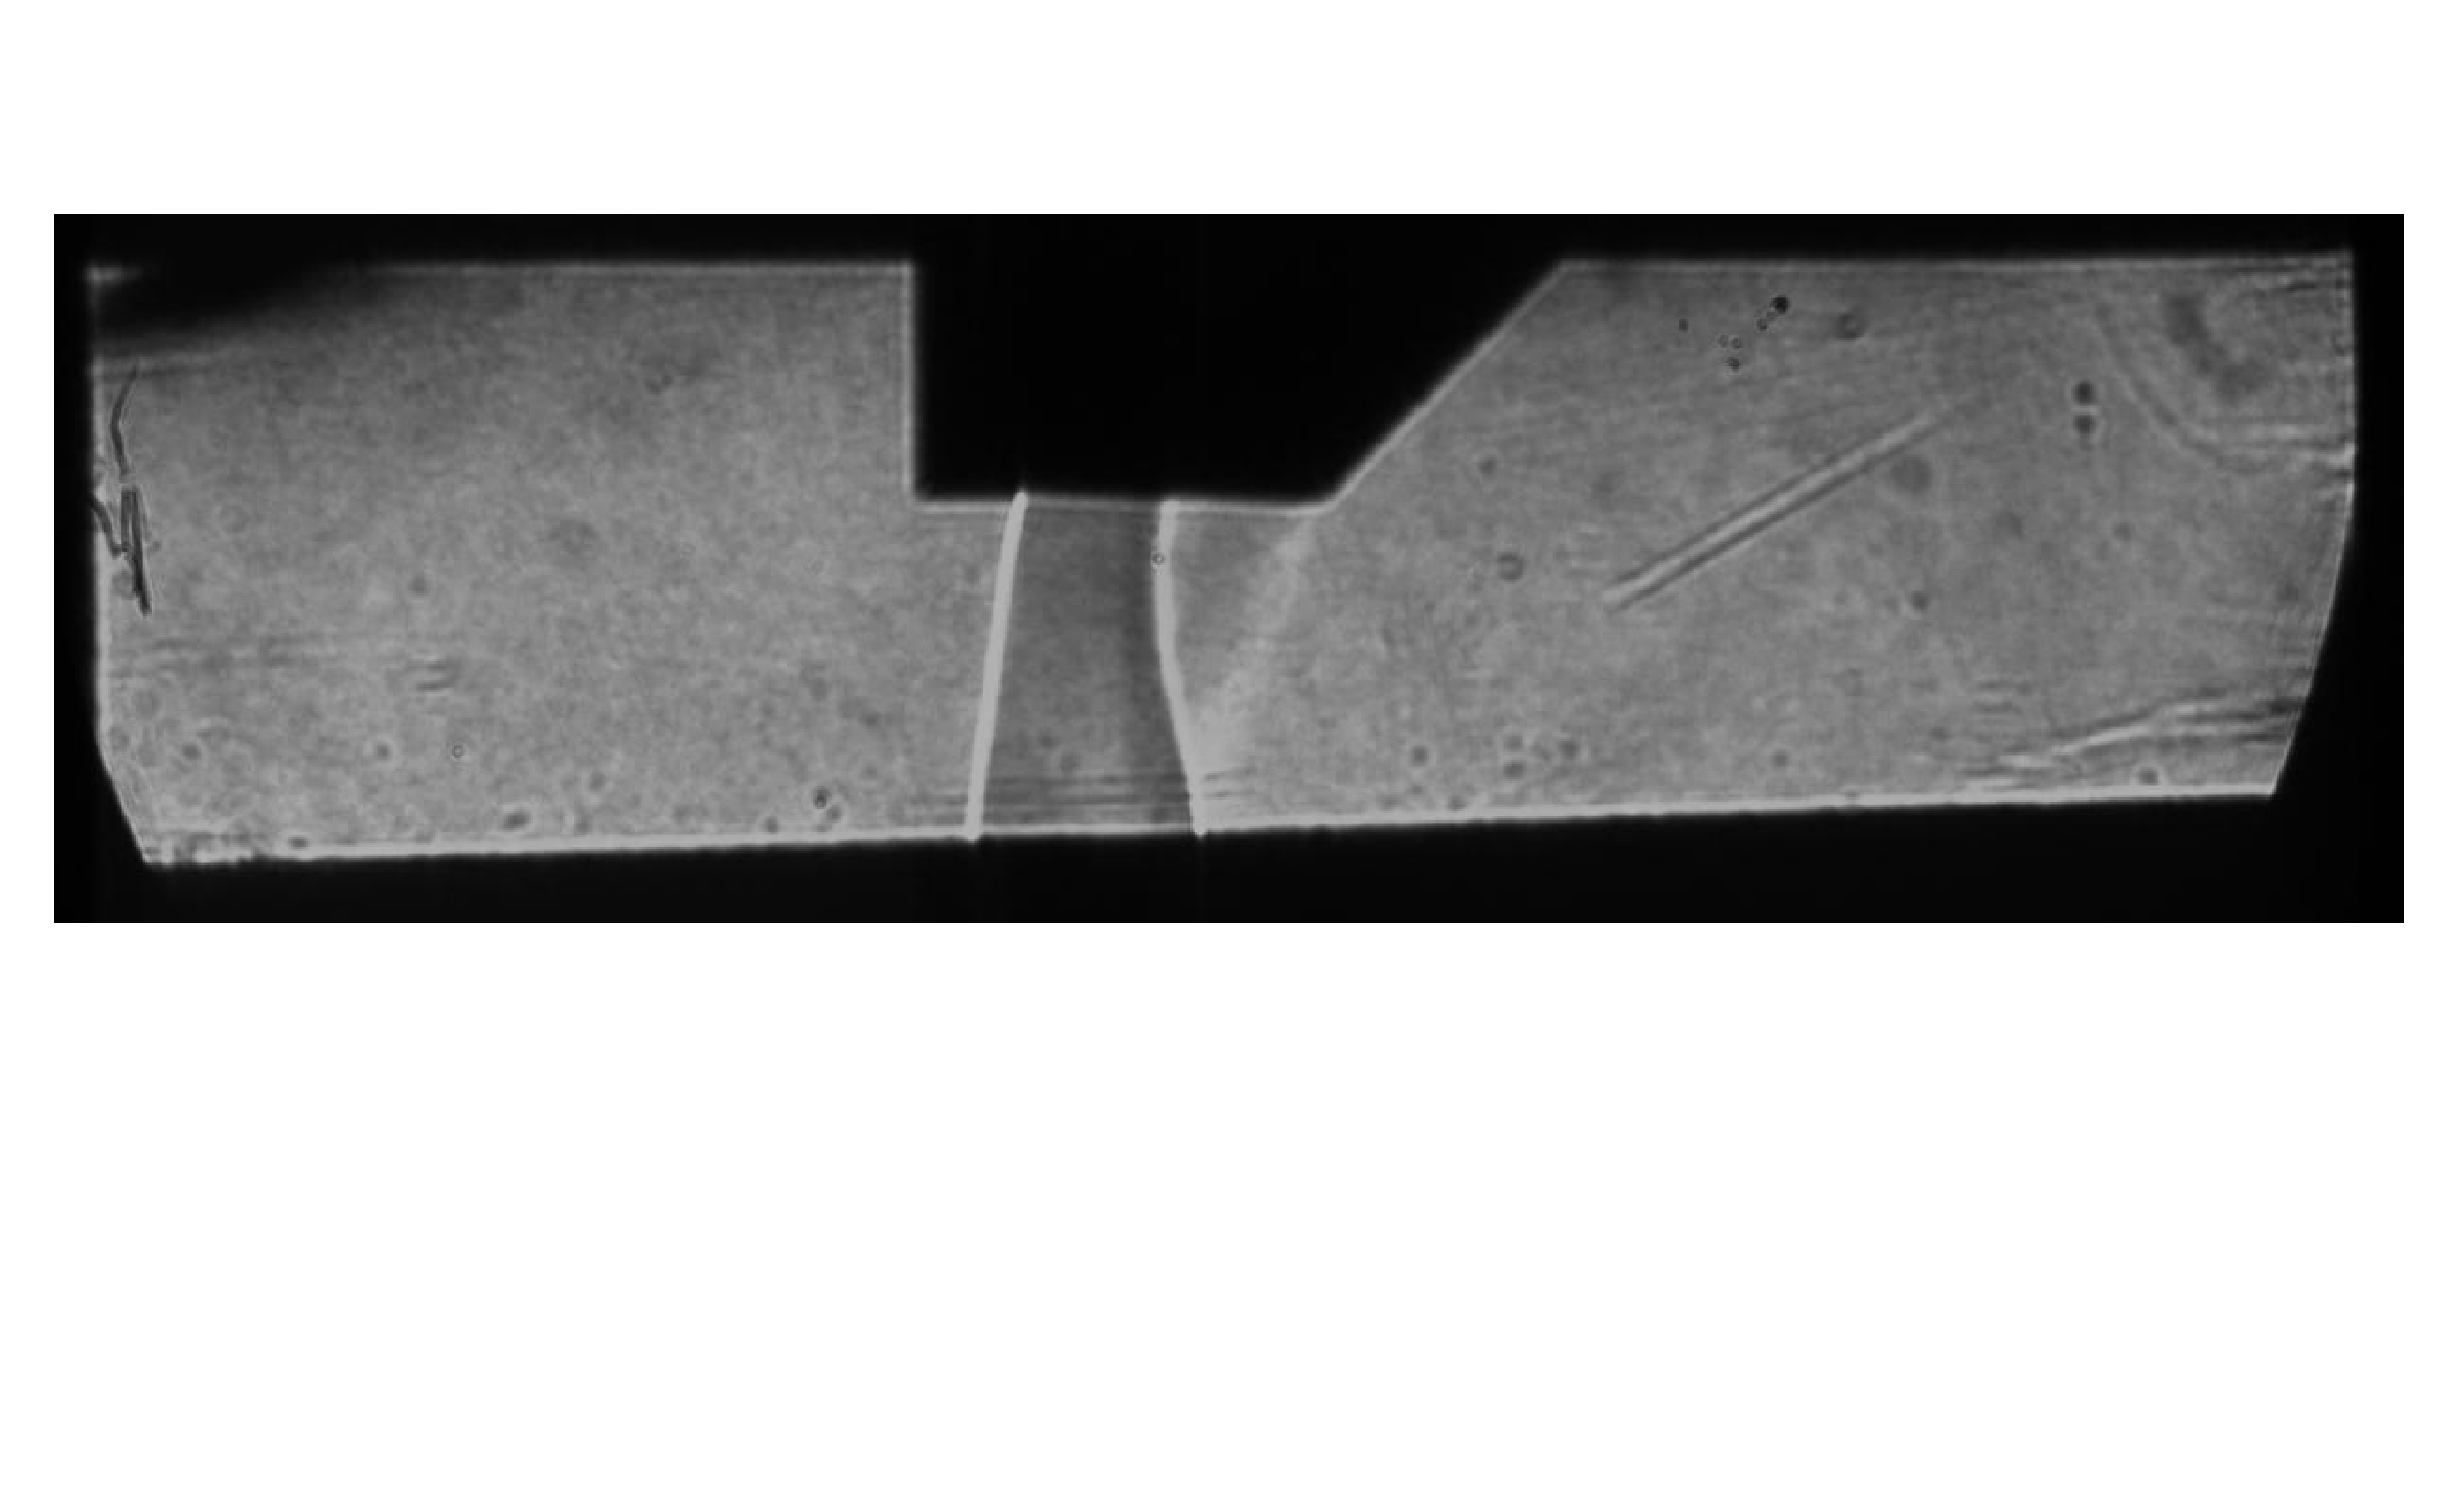
\includegraphics[width=0.99\textwidth]{shadow1of2.pdf}\\
(a)阴影法{\textcolor{white}{纵切1/2光线}}
\end{minipage}%
\begin{minipage}[b]{.5\textwidth}
\centering
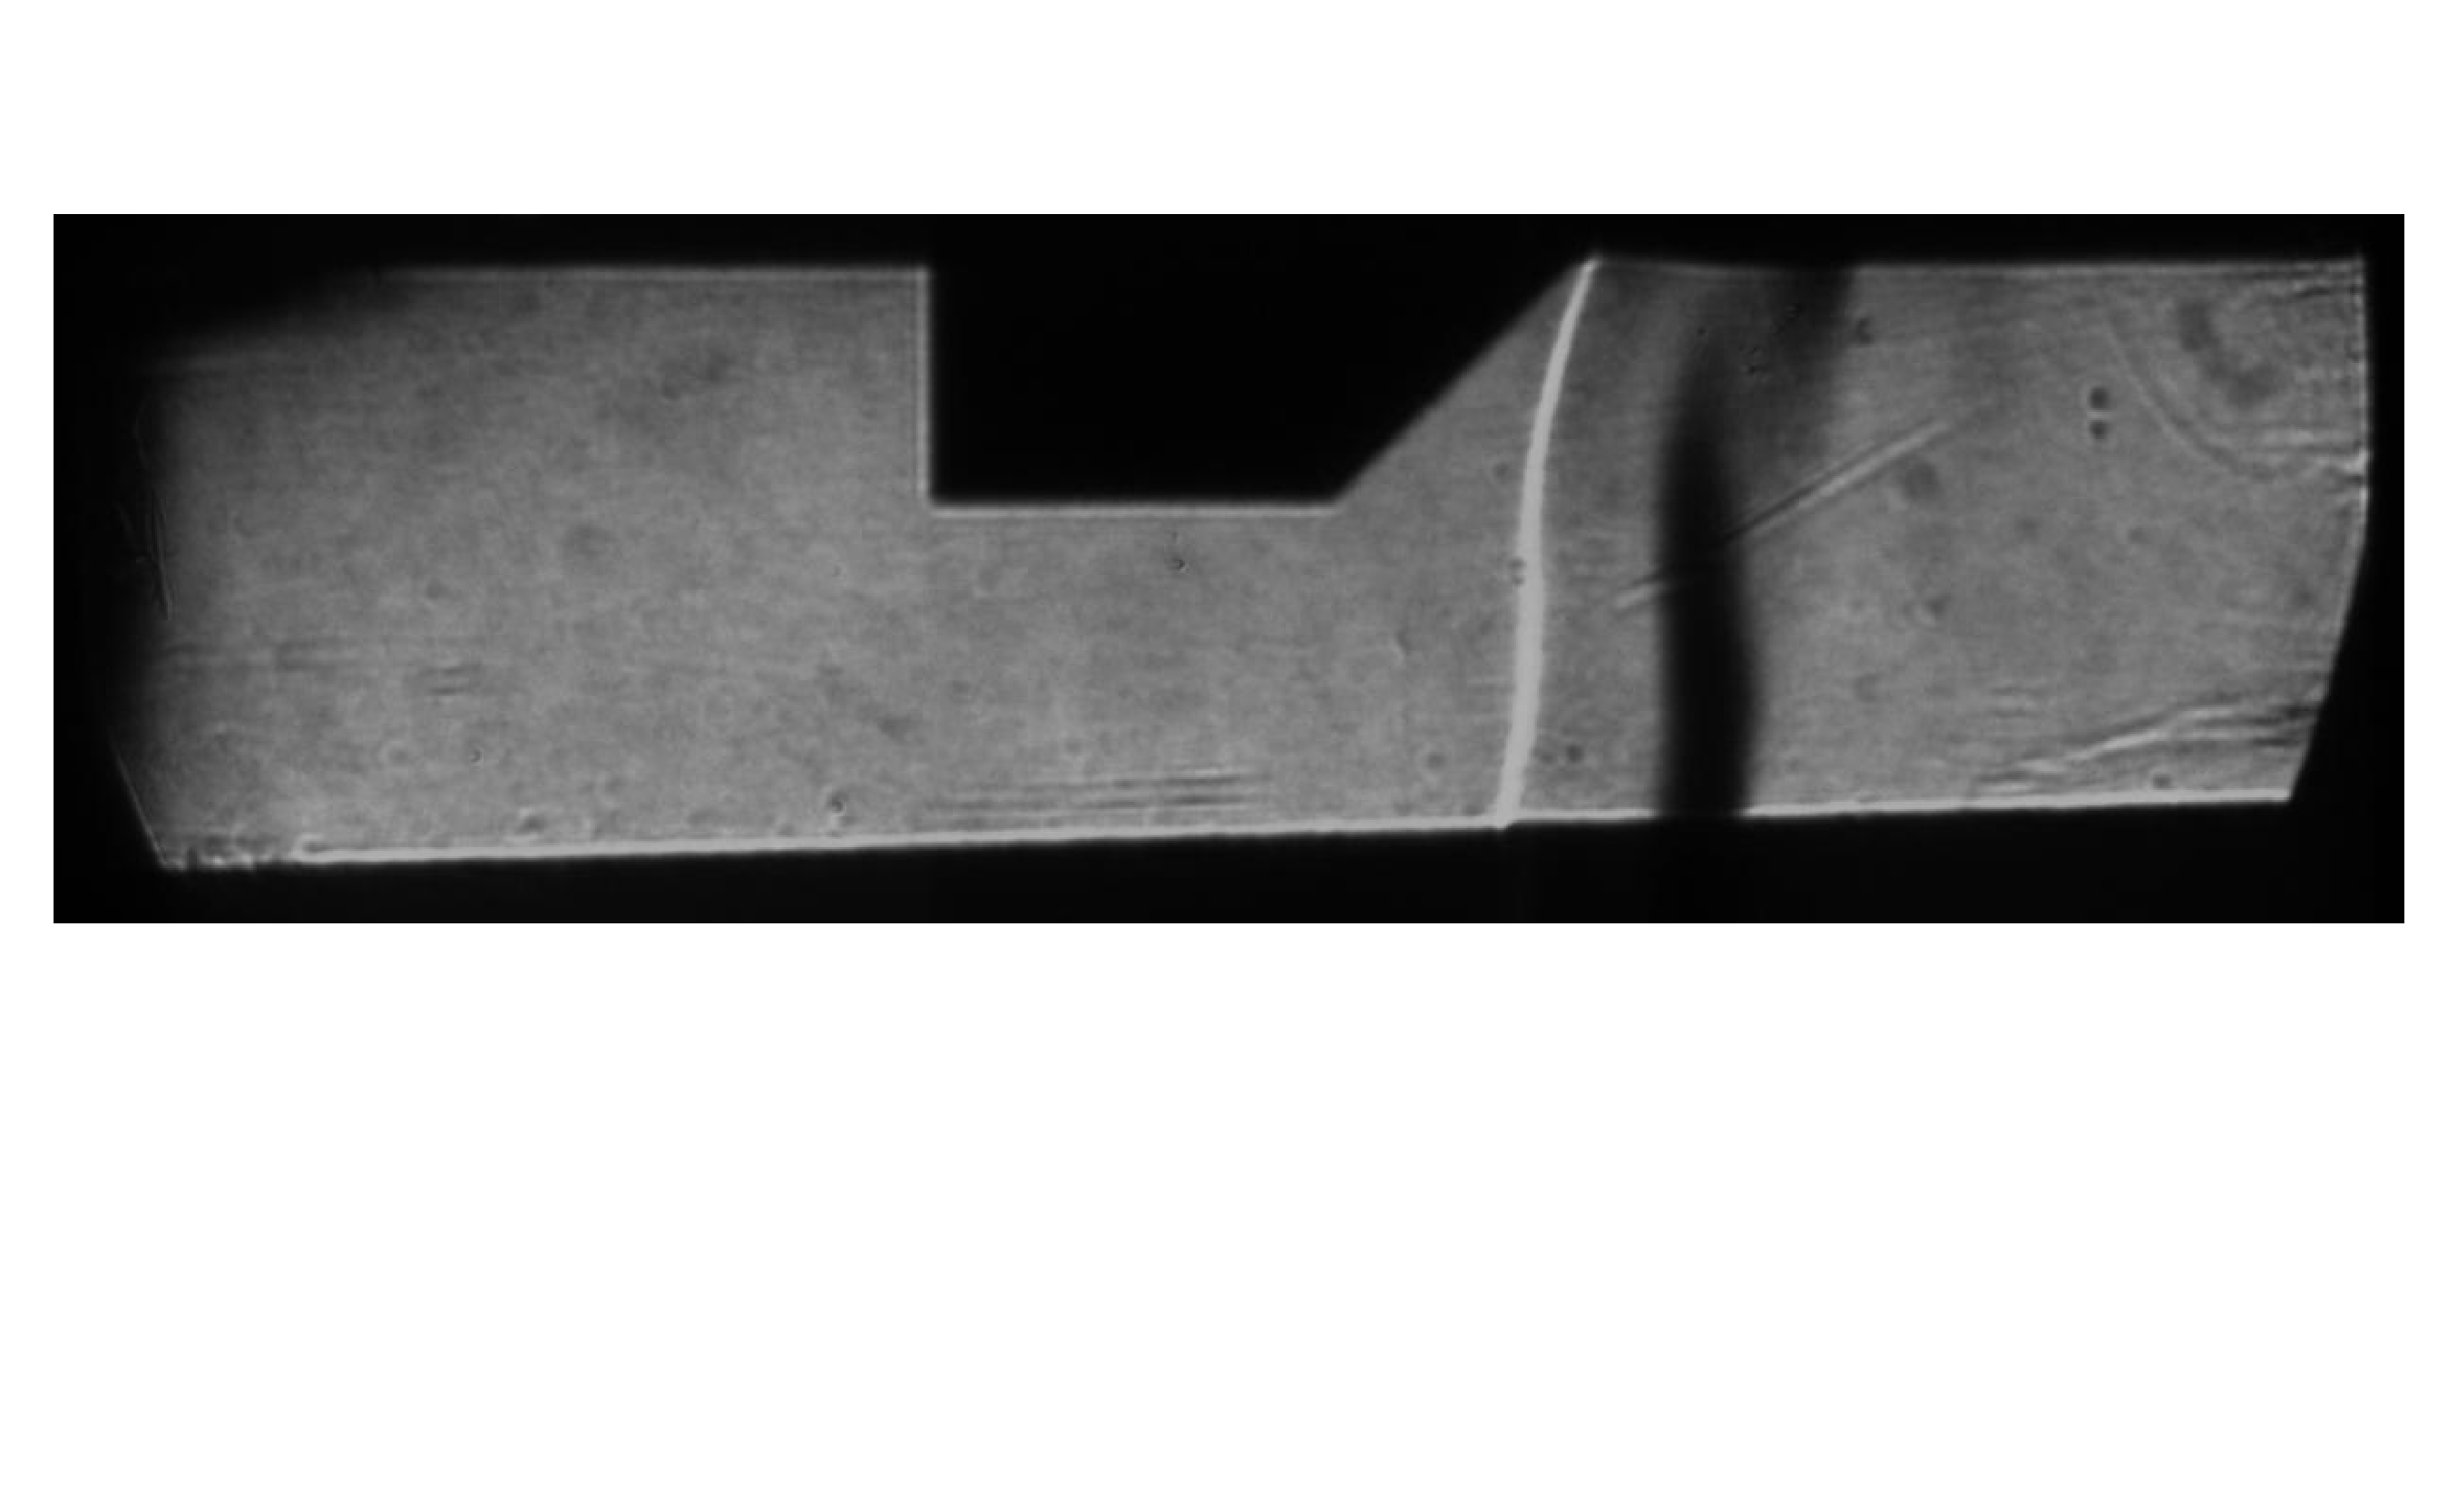
\includegraphics[width=0.99\textwidth]{fire-schlieren1of2.pdf}\\
(b)纹影法纵切1/2光线
\end{minipage}
\vspace{1em}

\begin{minipage}[b]{.5\textwidth}
\centering
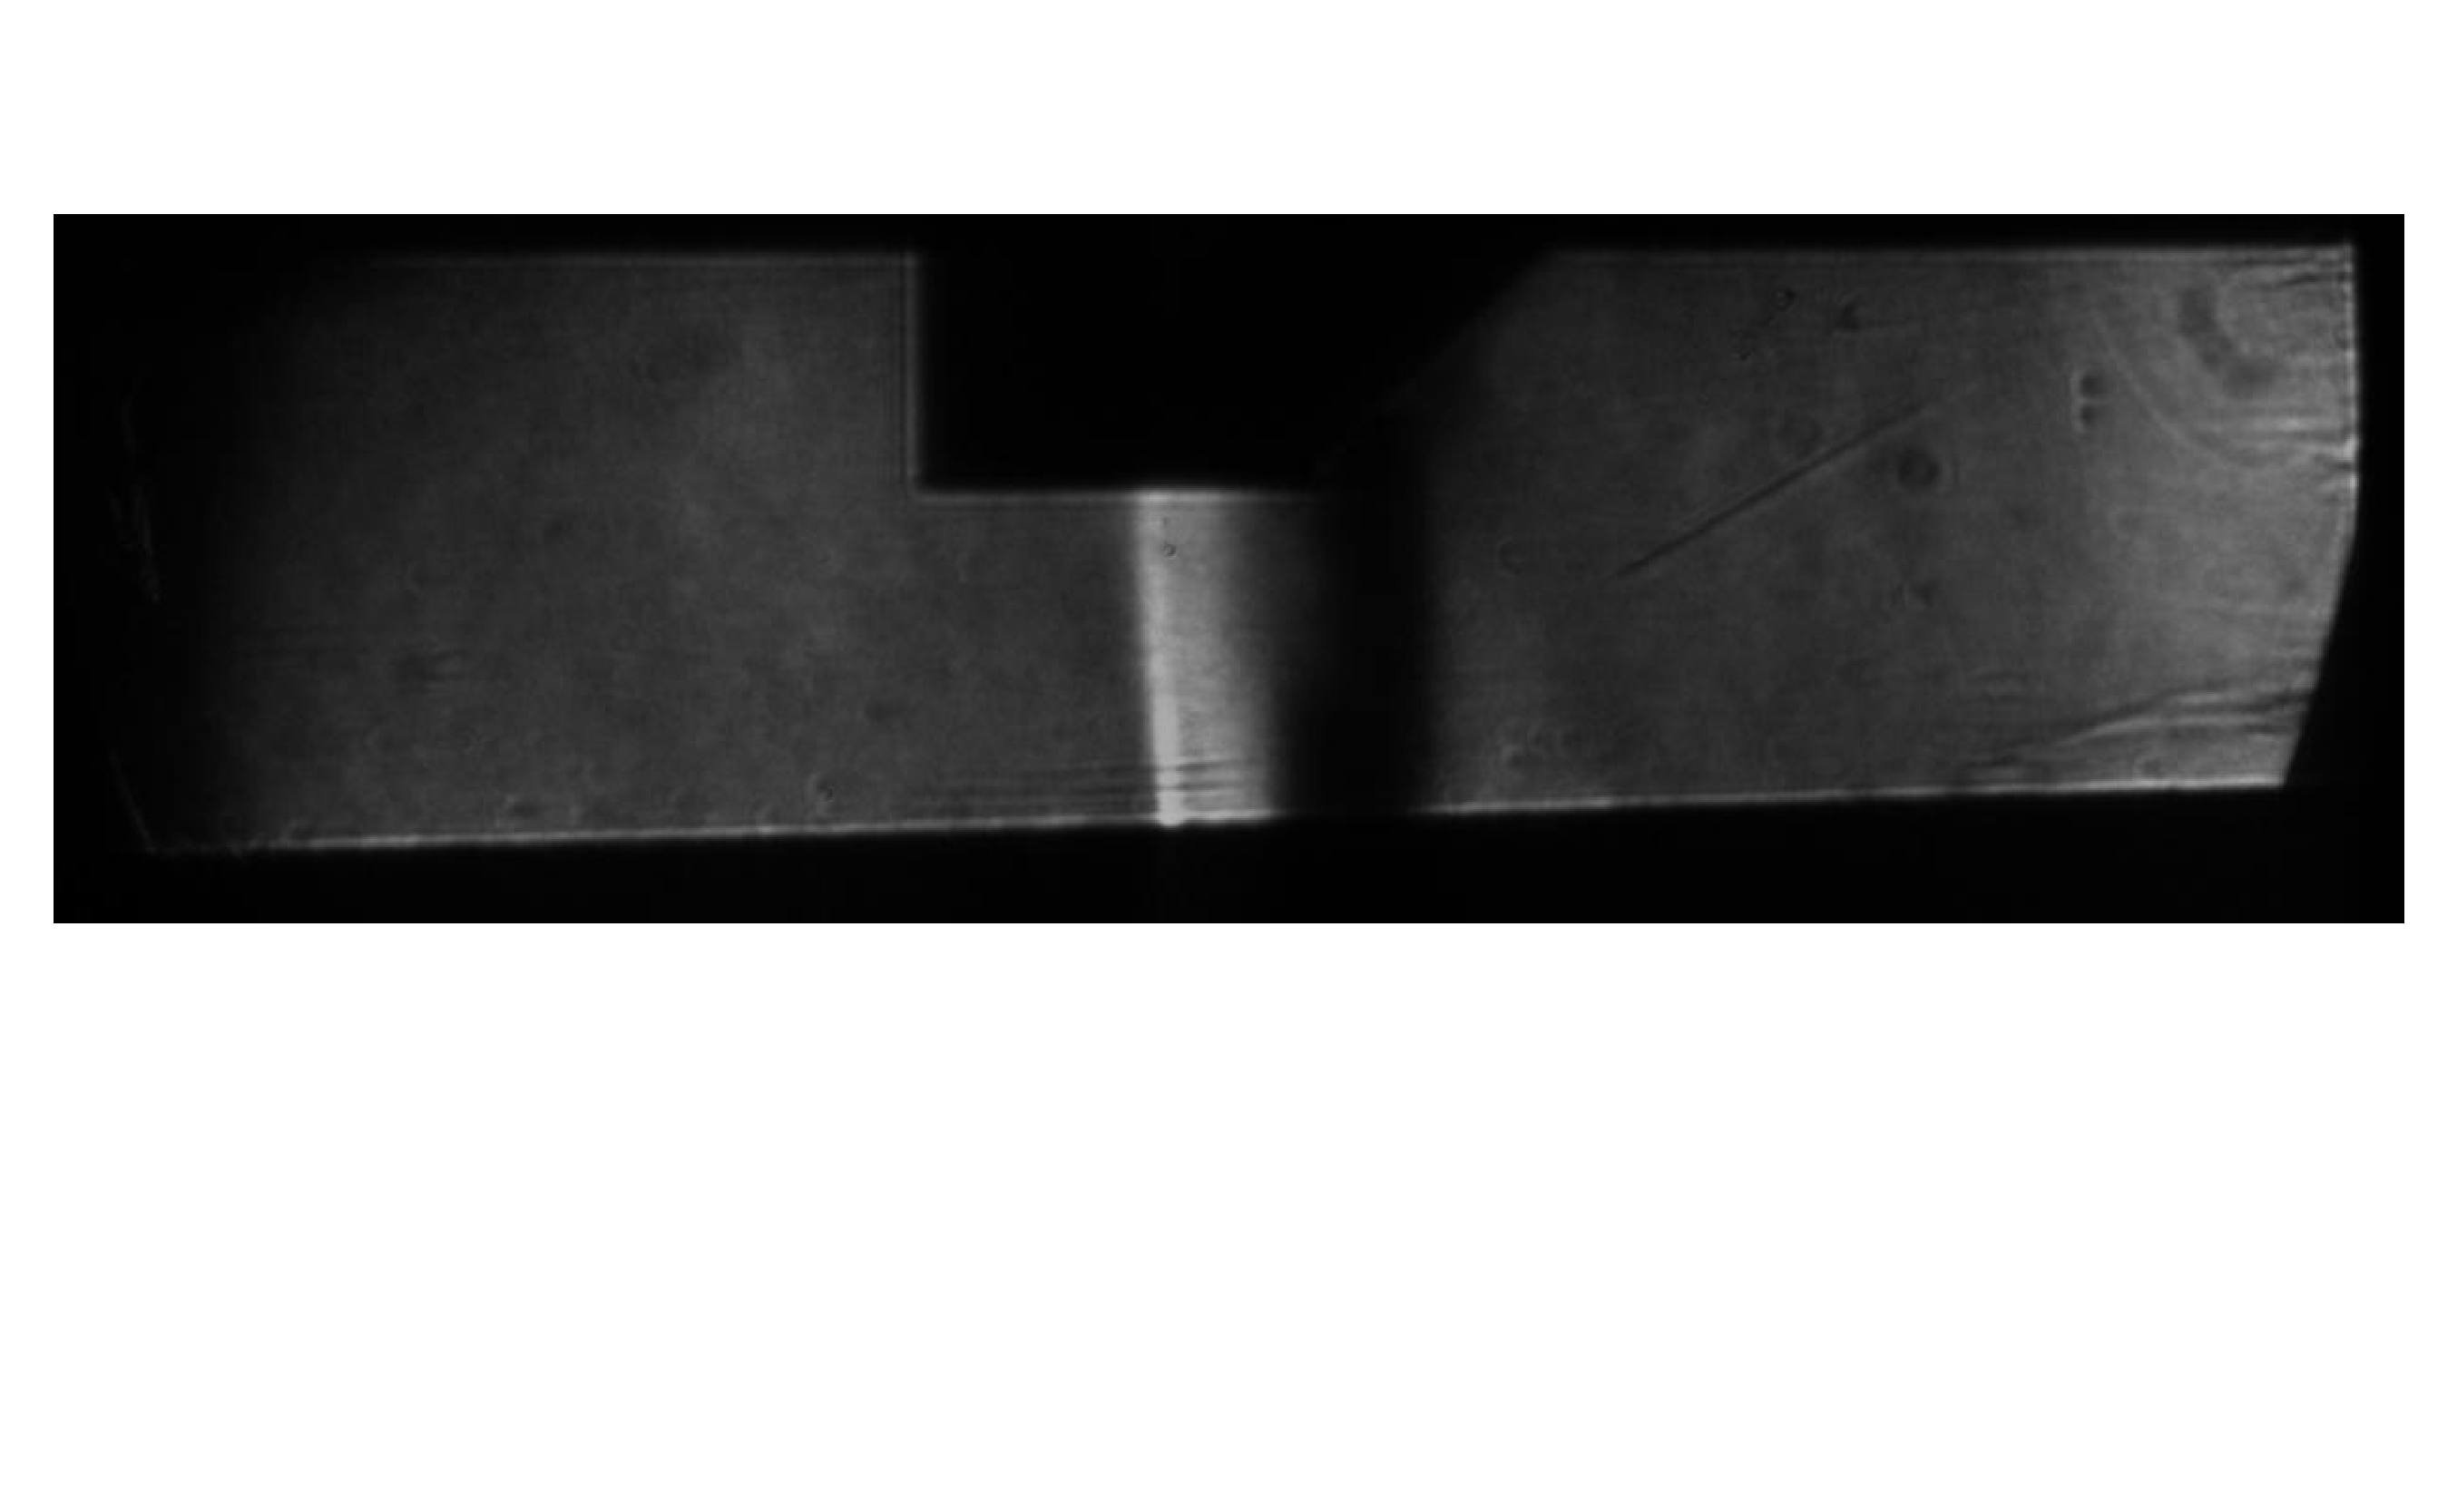
\includegraphics[width=0.99\textwidth]{fire-schlieren3of4.pdf}\\
(c)纹影法纵切3/4光线
\end{minipage}%
\begin{minipage}[b]{.5\textwidth}
\centering
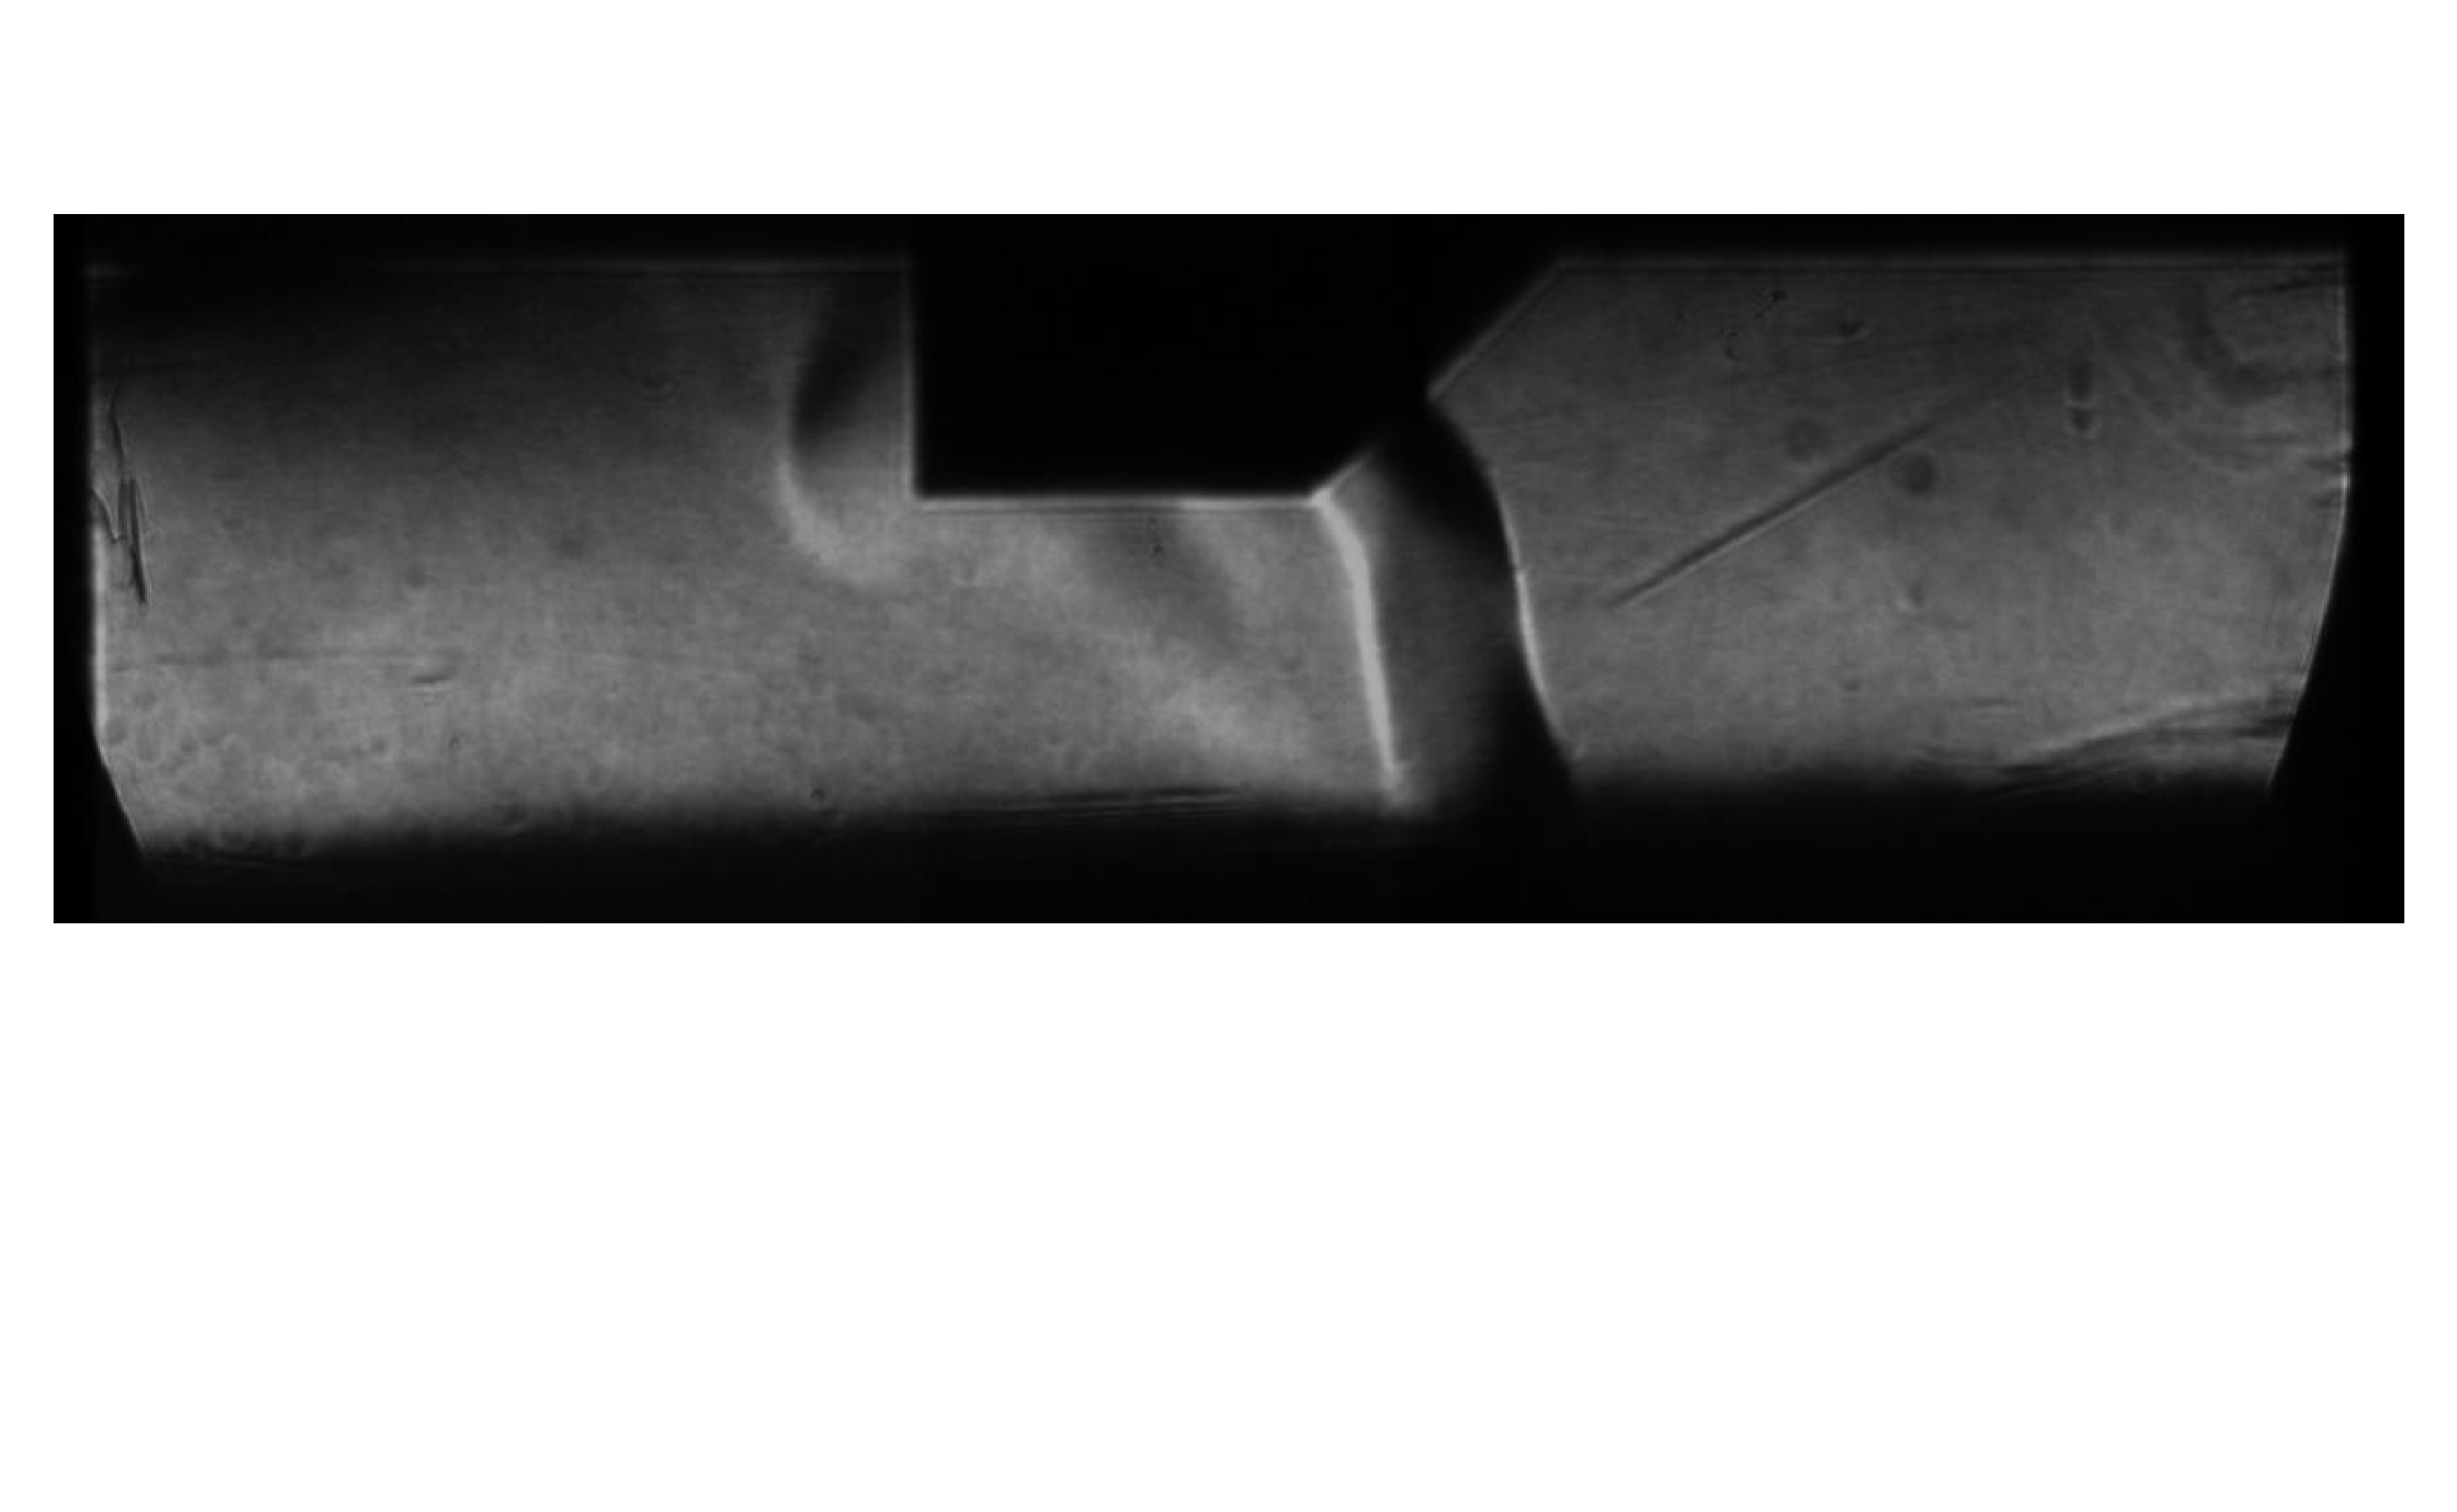
\includegraphics[width=0.99\textwidth]{fire-hschlieren1of2.pdf}\\
(d)纹影法横切1/2光线
\end{minipage}
}

%\frame{\frametitle{激波图案(视频)}
%\includemovie[poster, autostart, mouse, repeat]{4.2in}{1.2in}{./avi/wave.avi}
%\includemovie[poster, autostart, mouse]{4.2in}{1.2in}{./avi/wave.avi}
%}

\frame[<+->]{\frametitle{激波图案}
\begin{minipage}[b]{.5\textwidth}
\centering
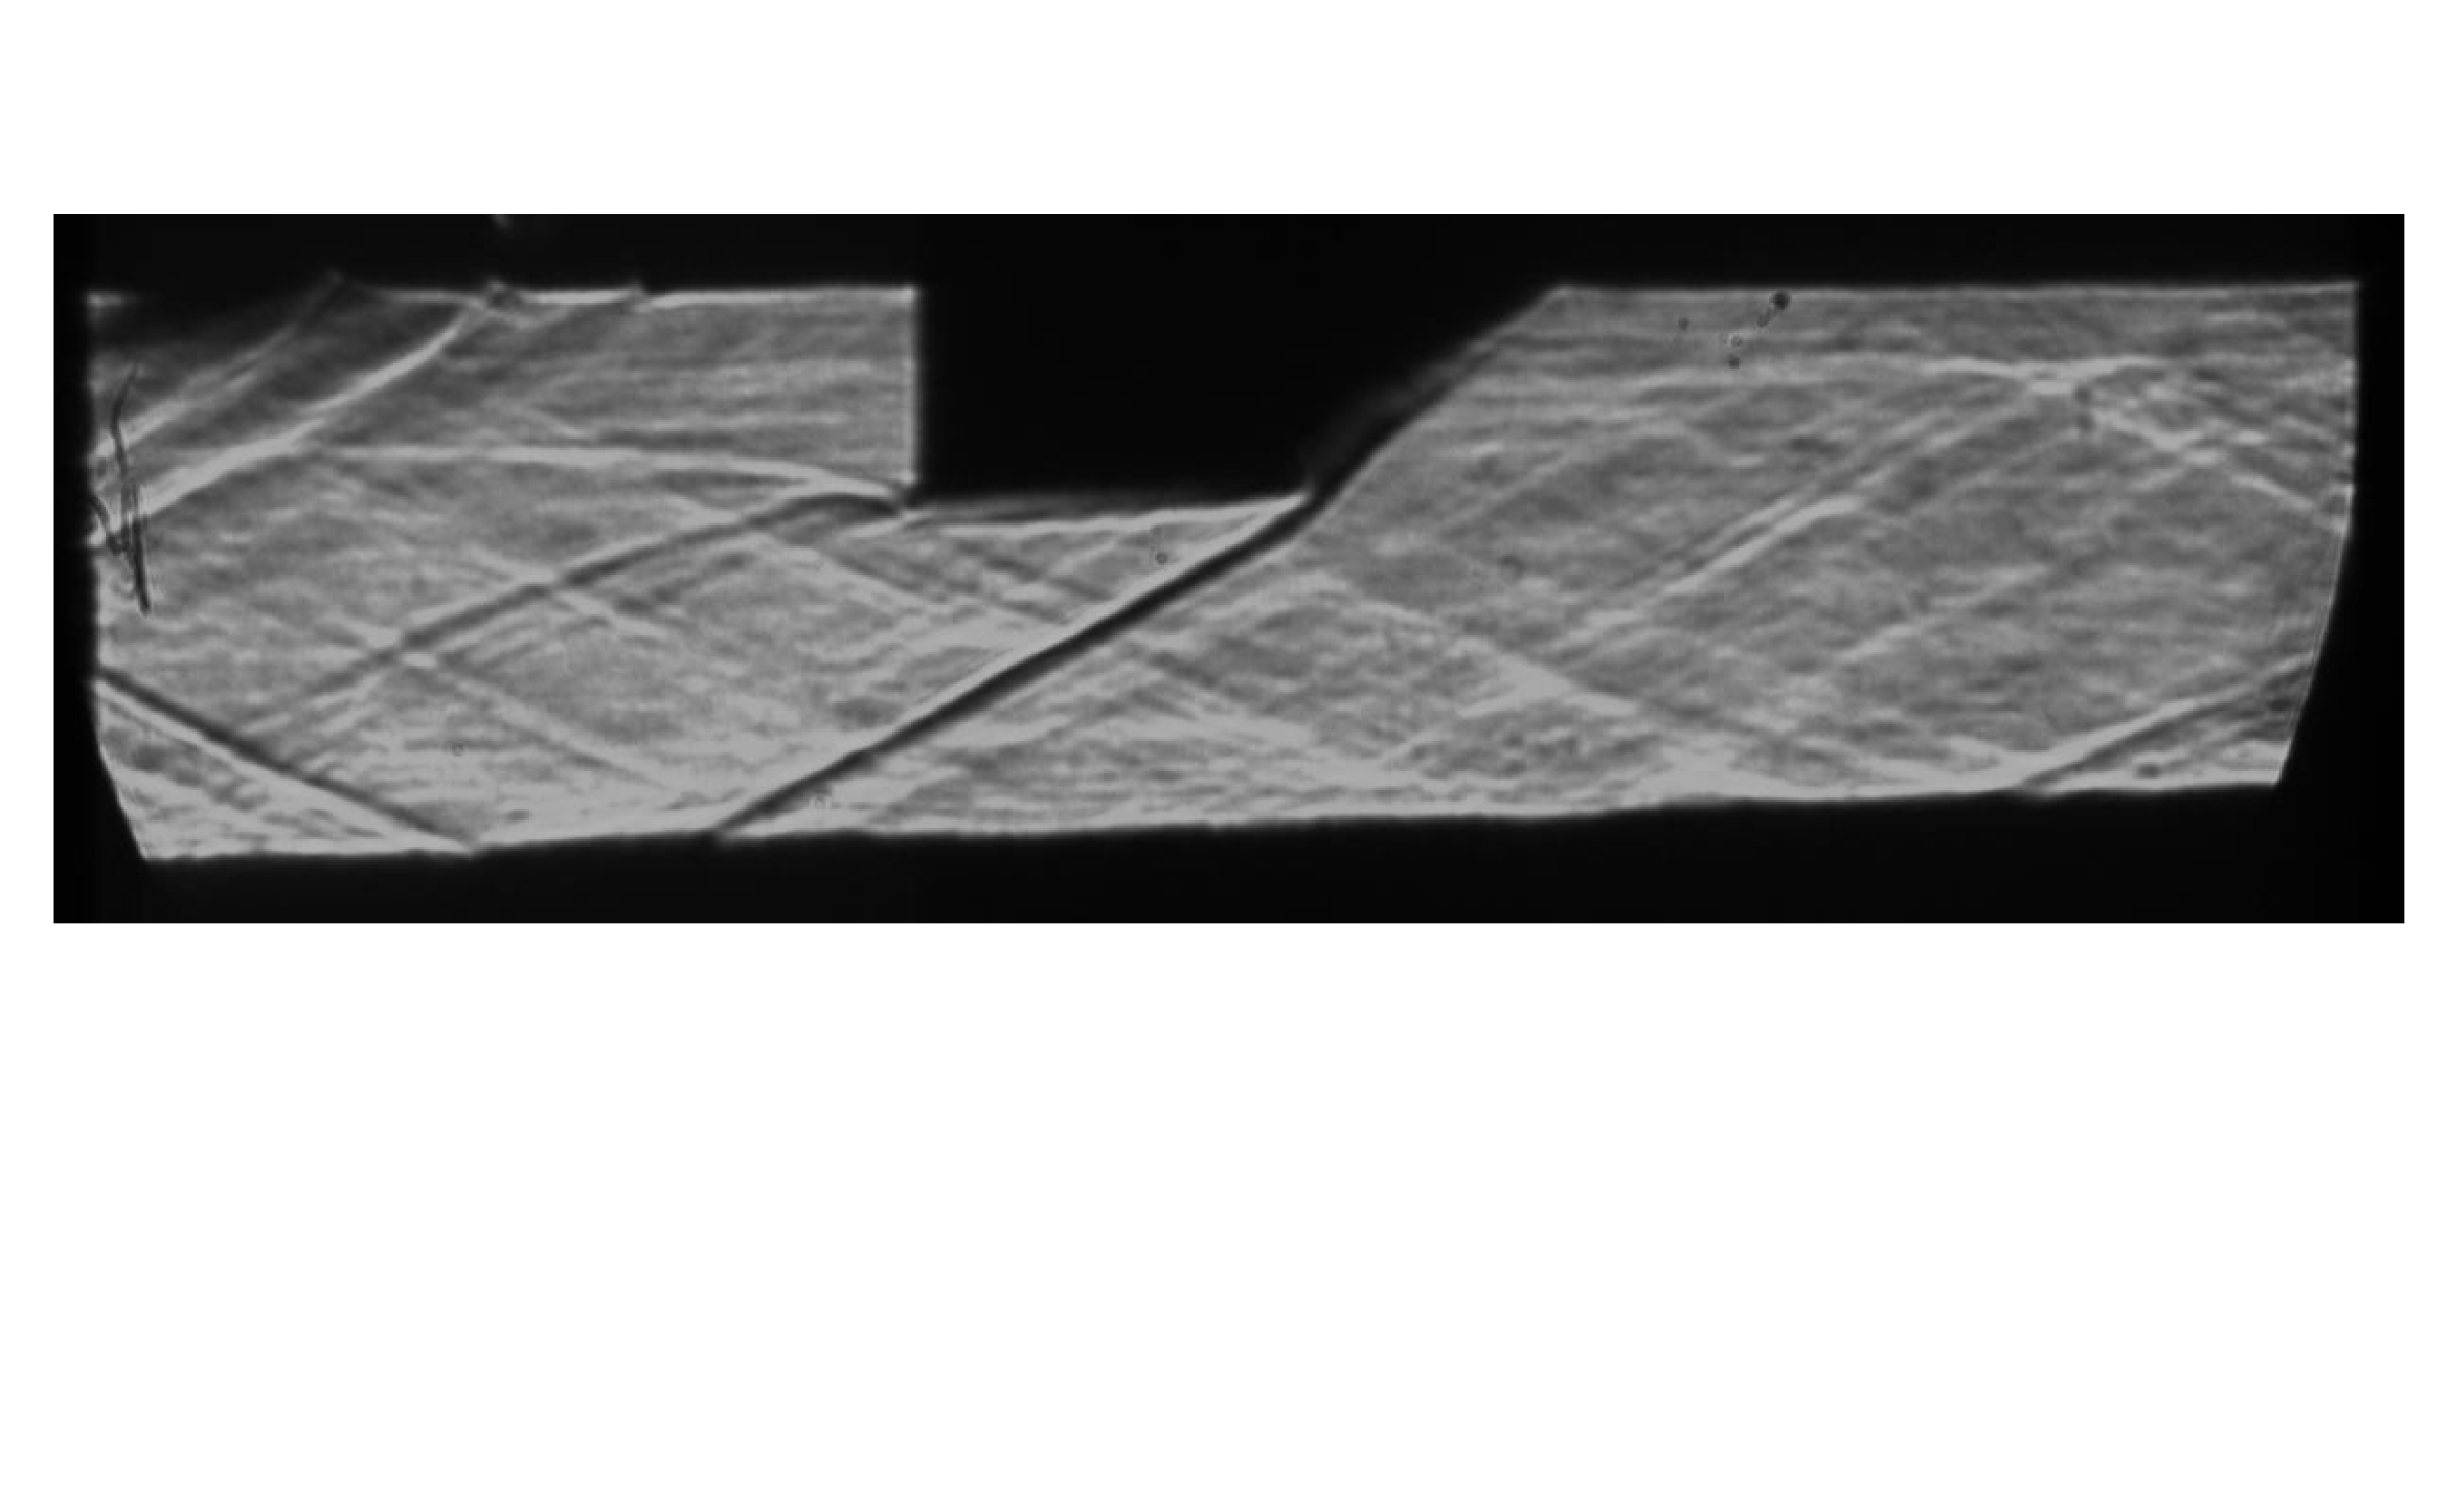
\includegraphics[width=0.99\textwidth]{WaveShadow.pdf}\\
(a)阴影法{\textcolor{white}{纵切1/2光线}}
\end{minipage}%
\begin{minipage}[b]{.5\textwidth}
\centering
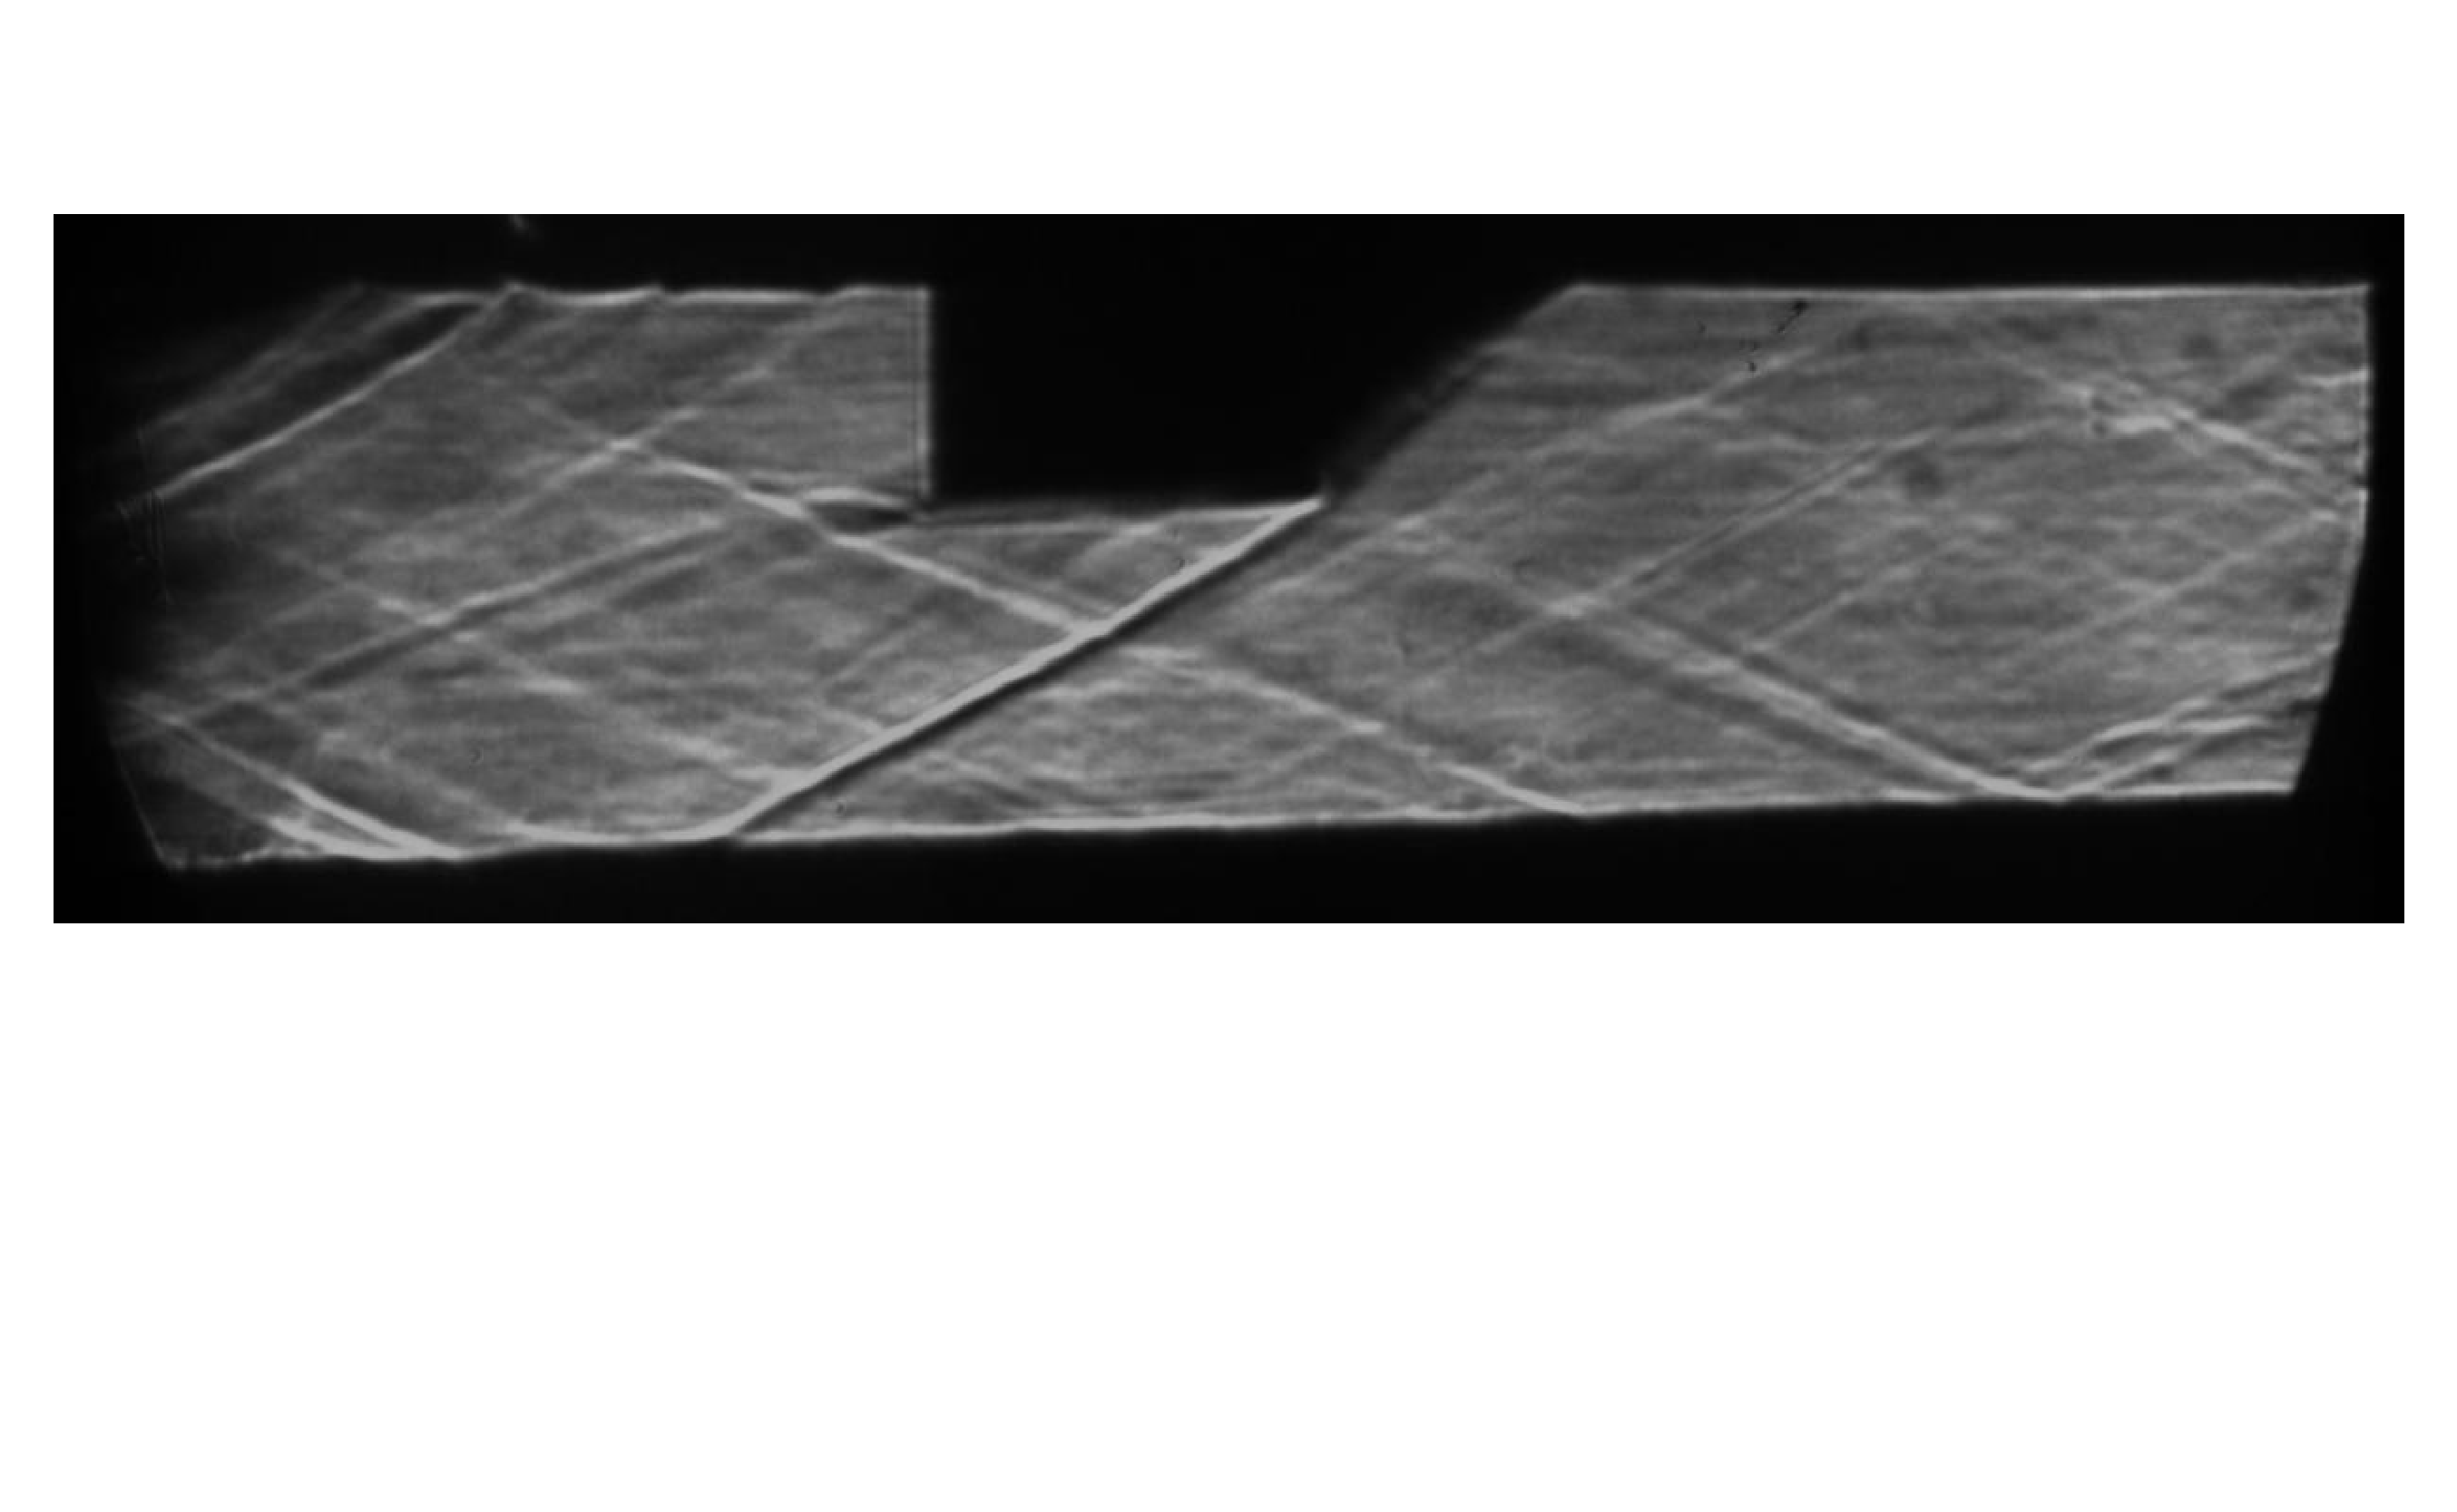
\includegraphics[width=0.99\textwidth]{WaveSchlieren1of2.pdf}\\
(b)纹影法纵切1/2光线
\end{minipage}
\vspace{1em}

\begin{minipage}[b]{.5\textwidth}
\centering
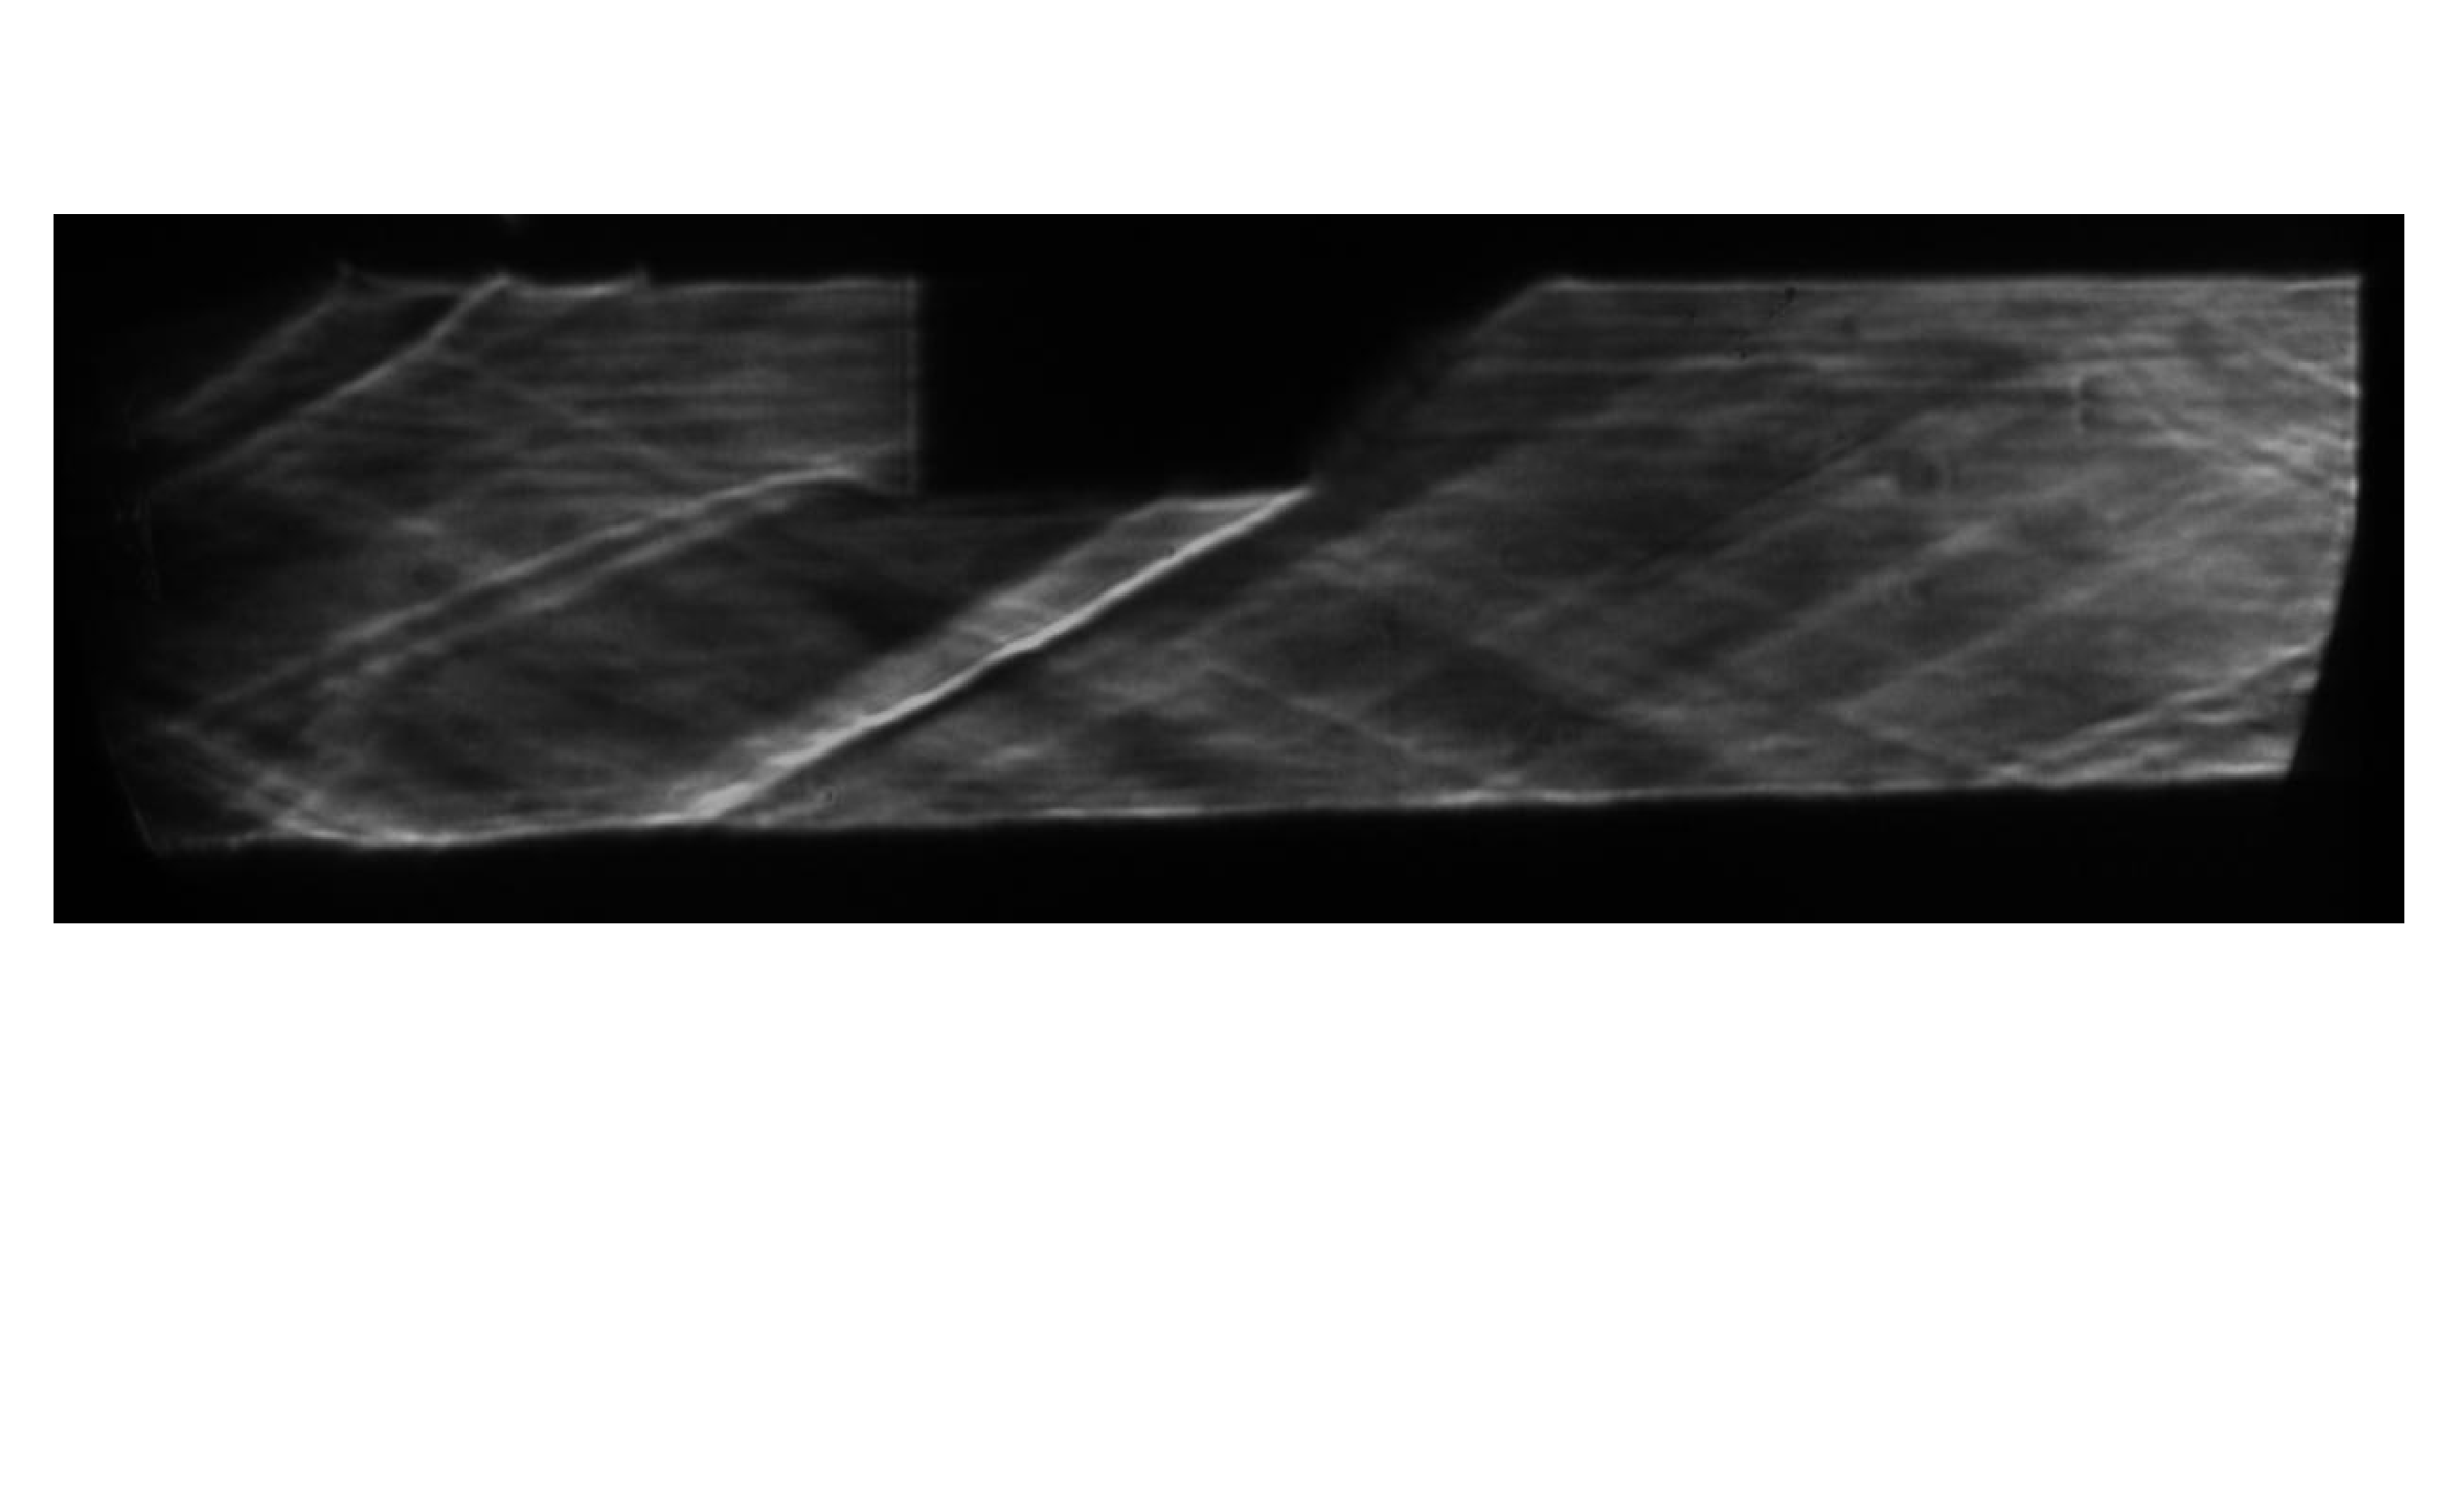
\includegraphics[width=0.99\textwidth]{WaveSchlieren3of4.pdf}\\
(c)纹影法纵切3/4光线
\end{minipage}%
\begin{minipage}[b]{.5\textwidth}
\centering
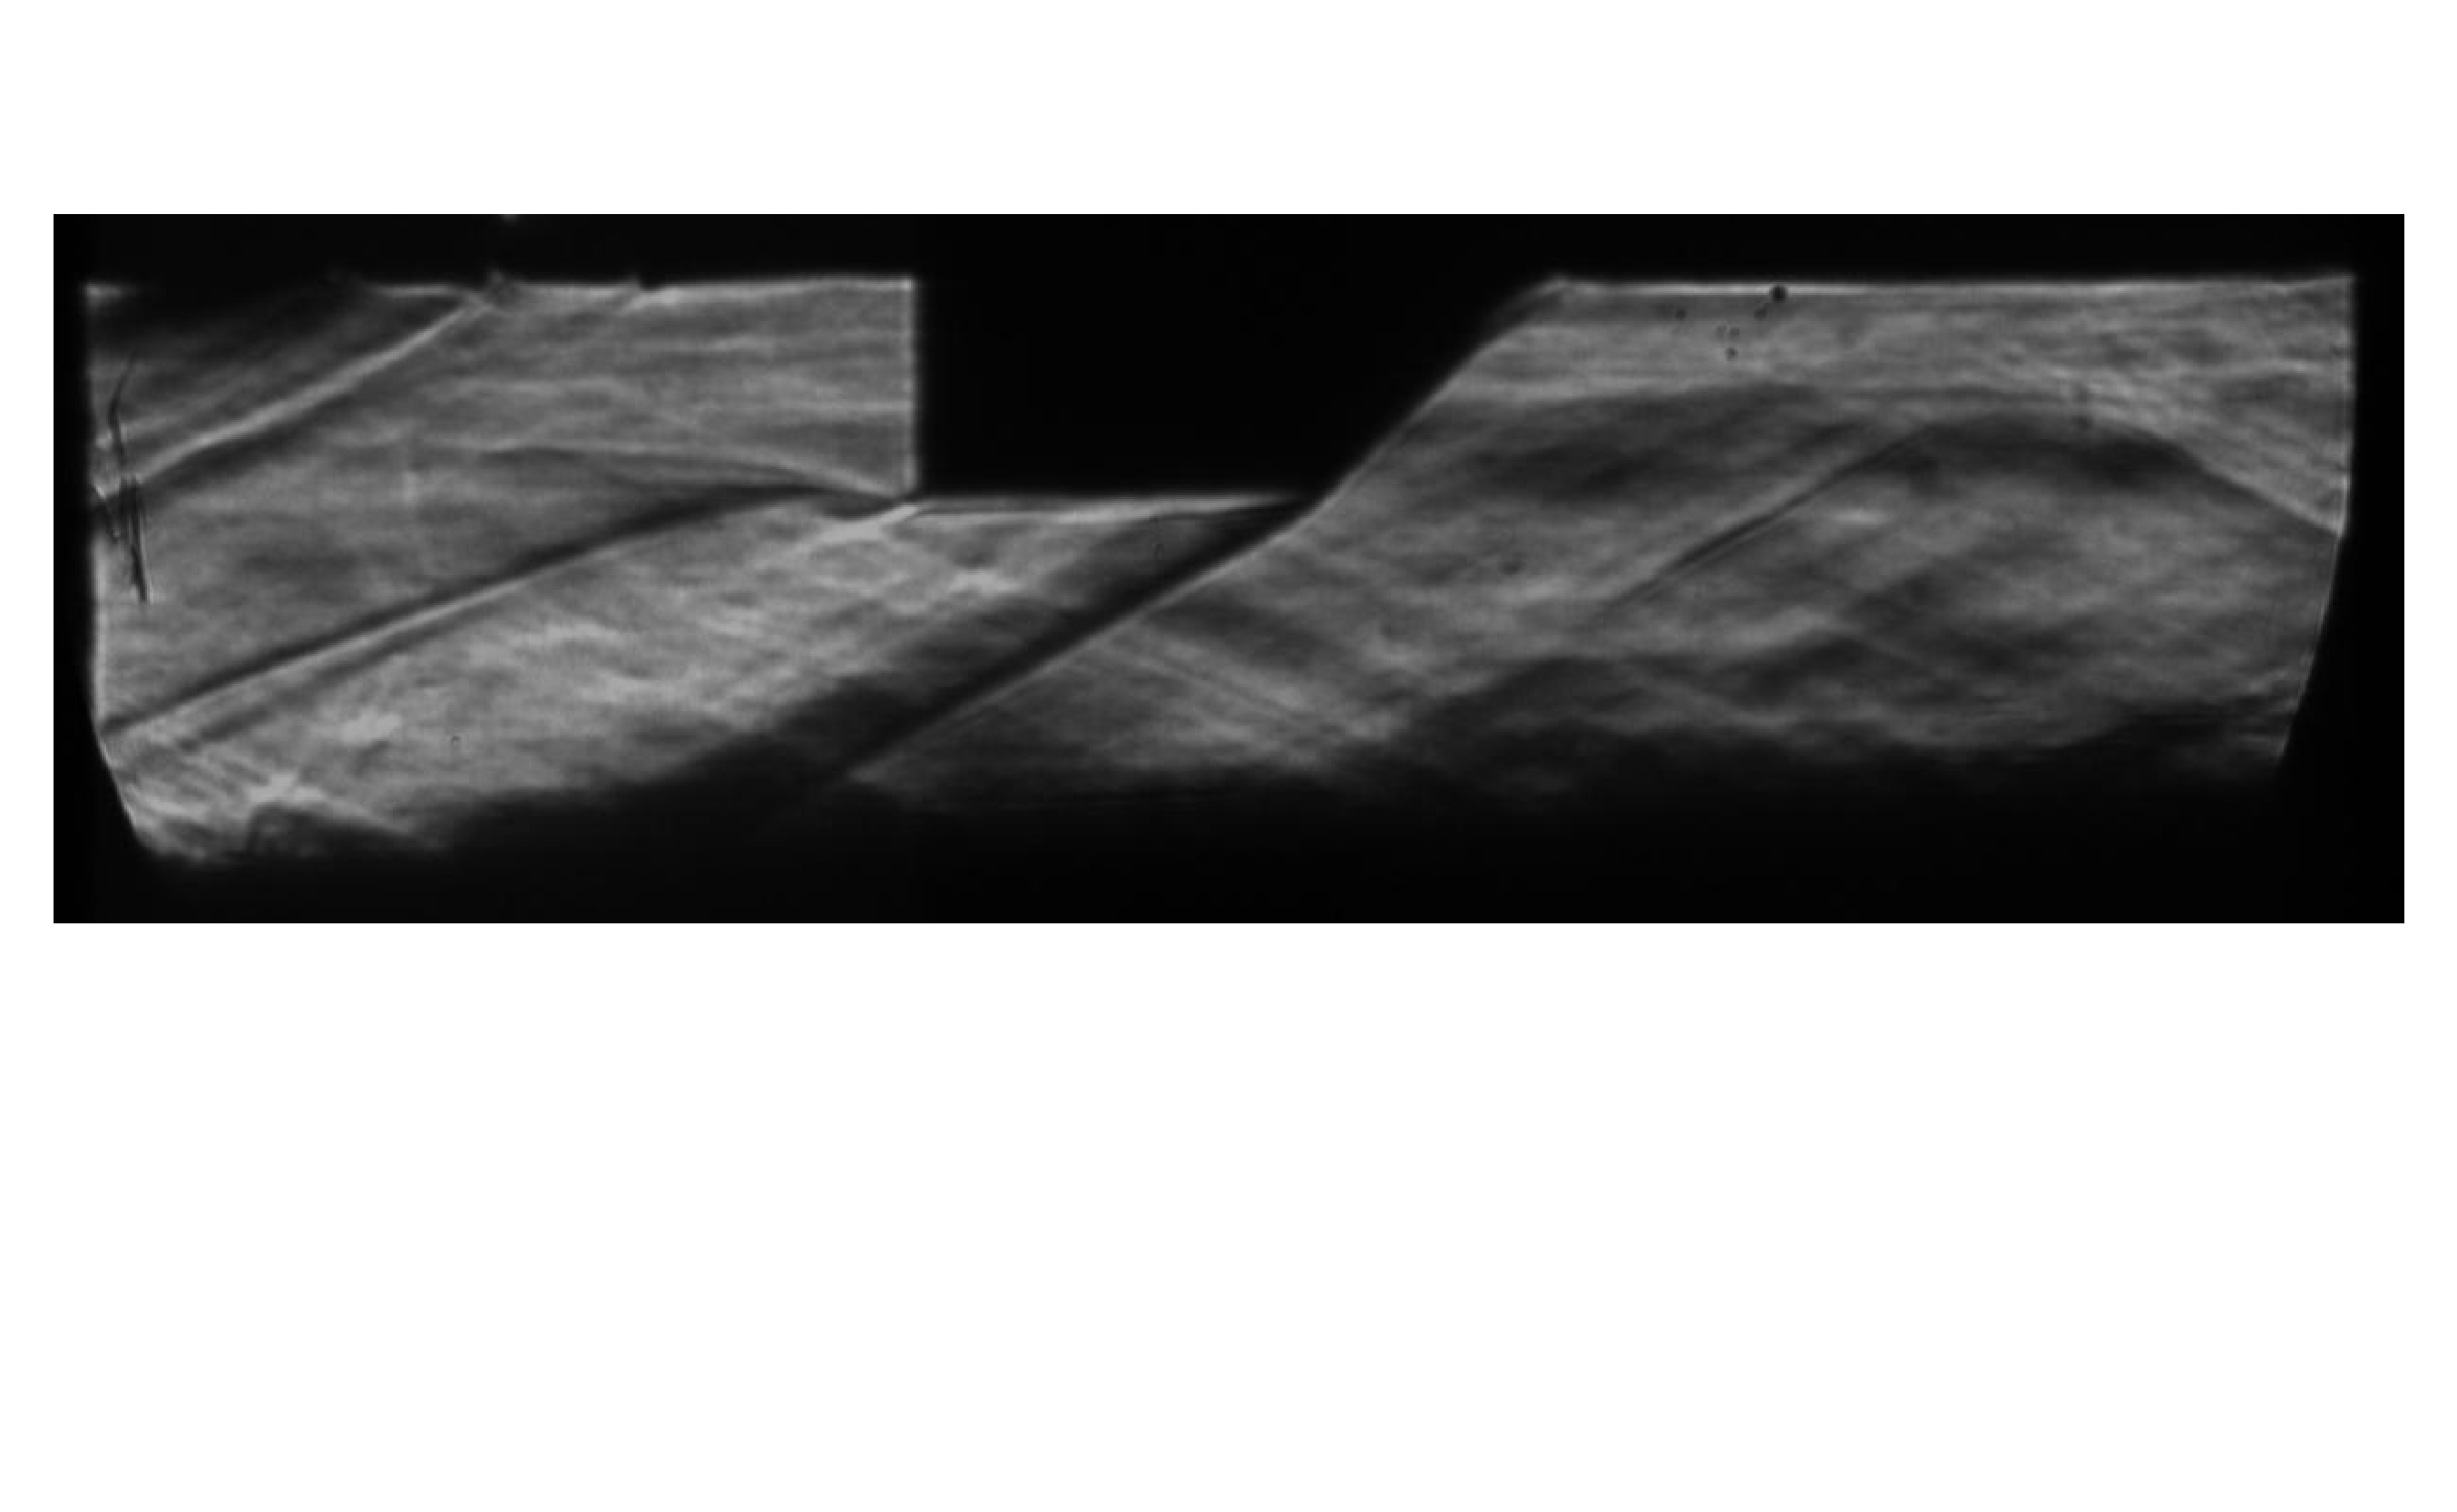
\includegraphics[width=0.99\textwidth]{WaveHSchlieren1of2.pdf}\\
(d)纹影法横切1/2光线
\end{minipage}
}

\subsection{结果分析}
\frame{\frametitle{波的类型与出现原因}
\begin{center}
\fbox{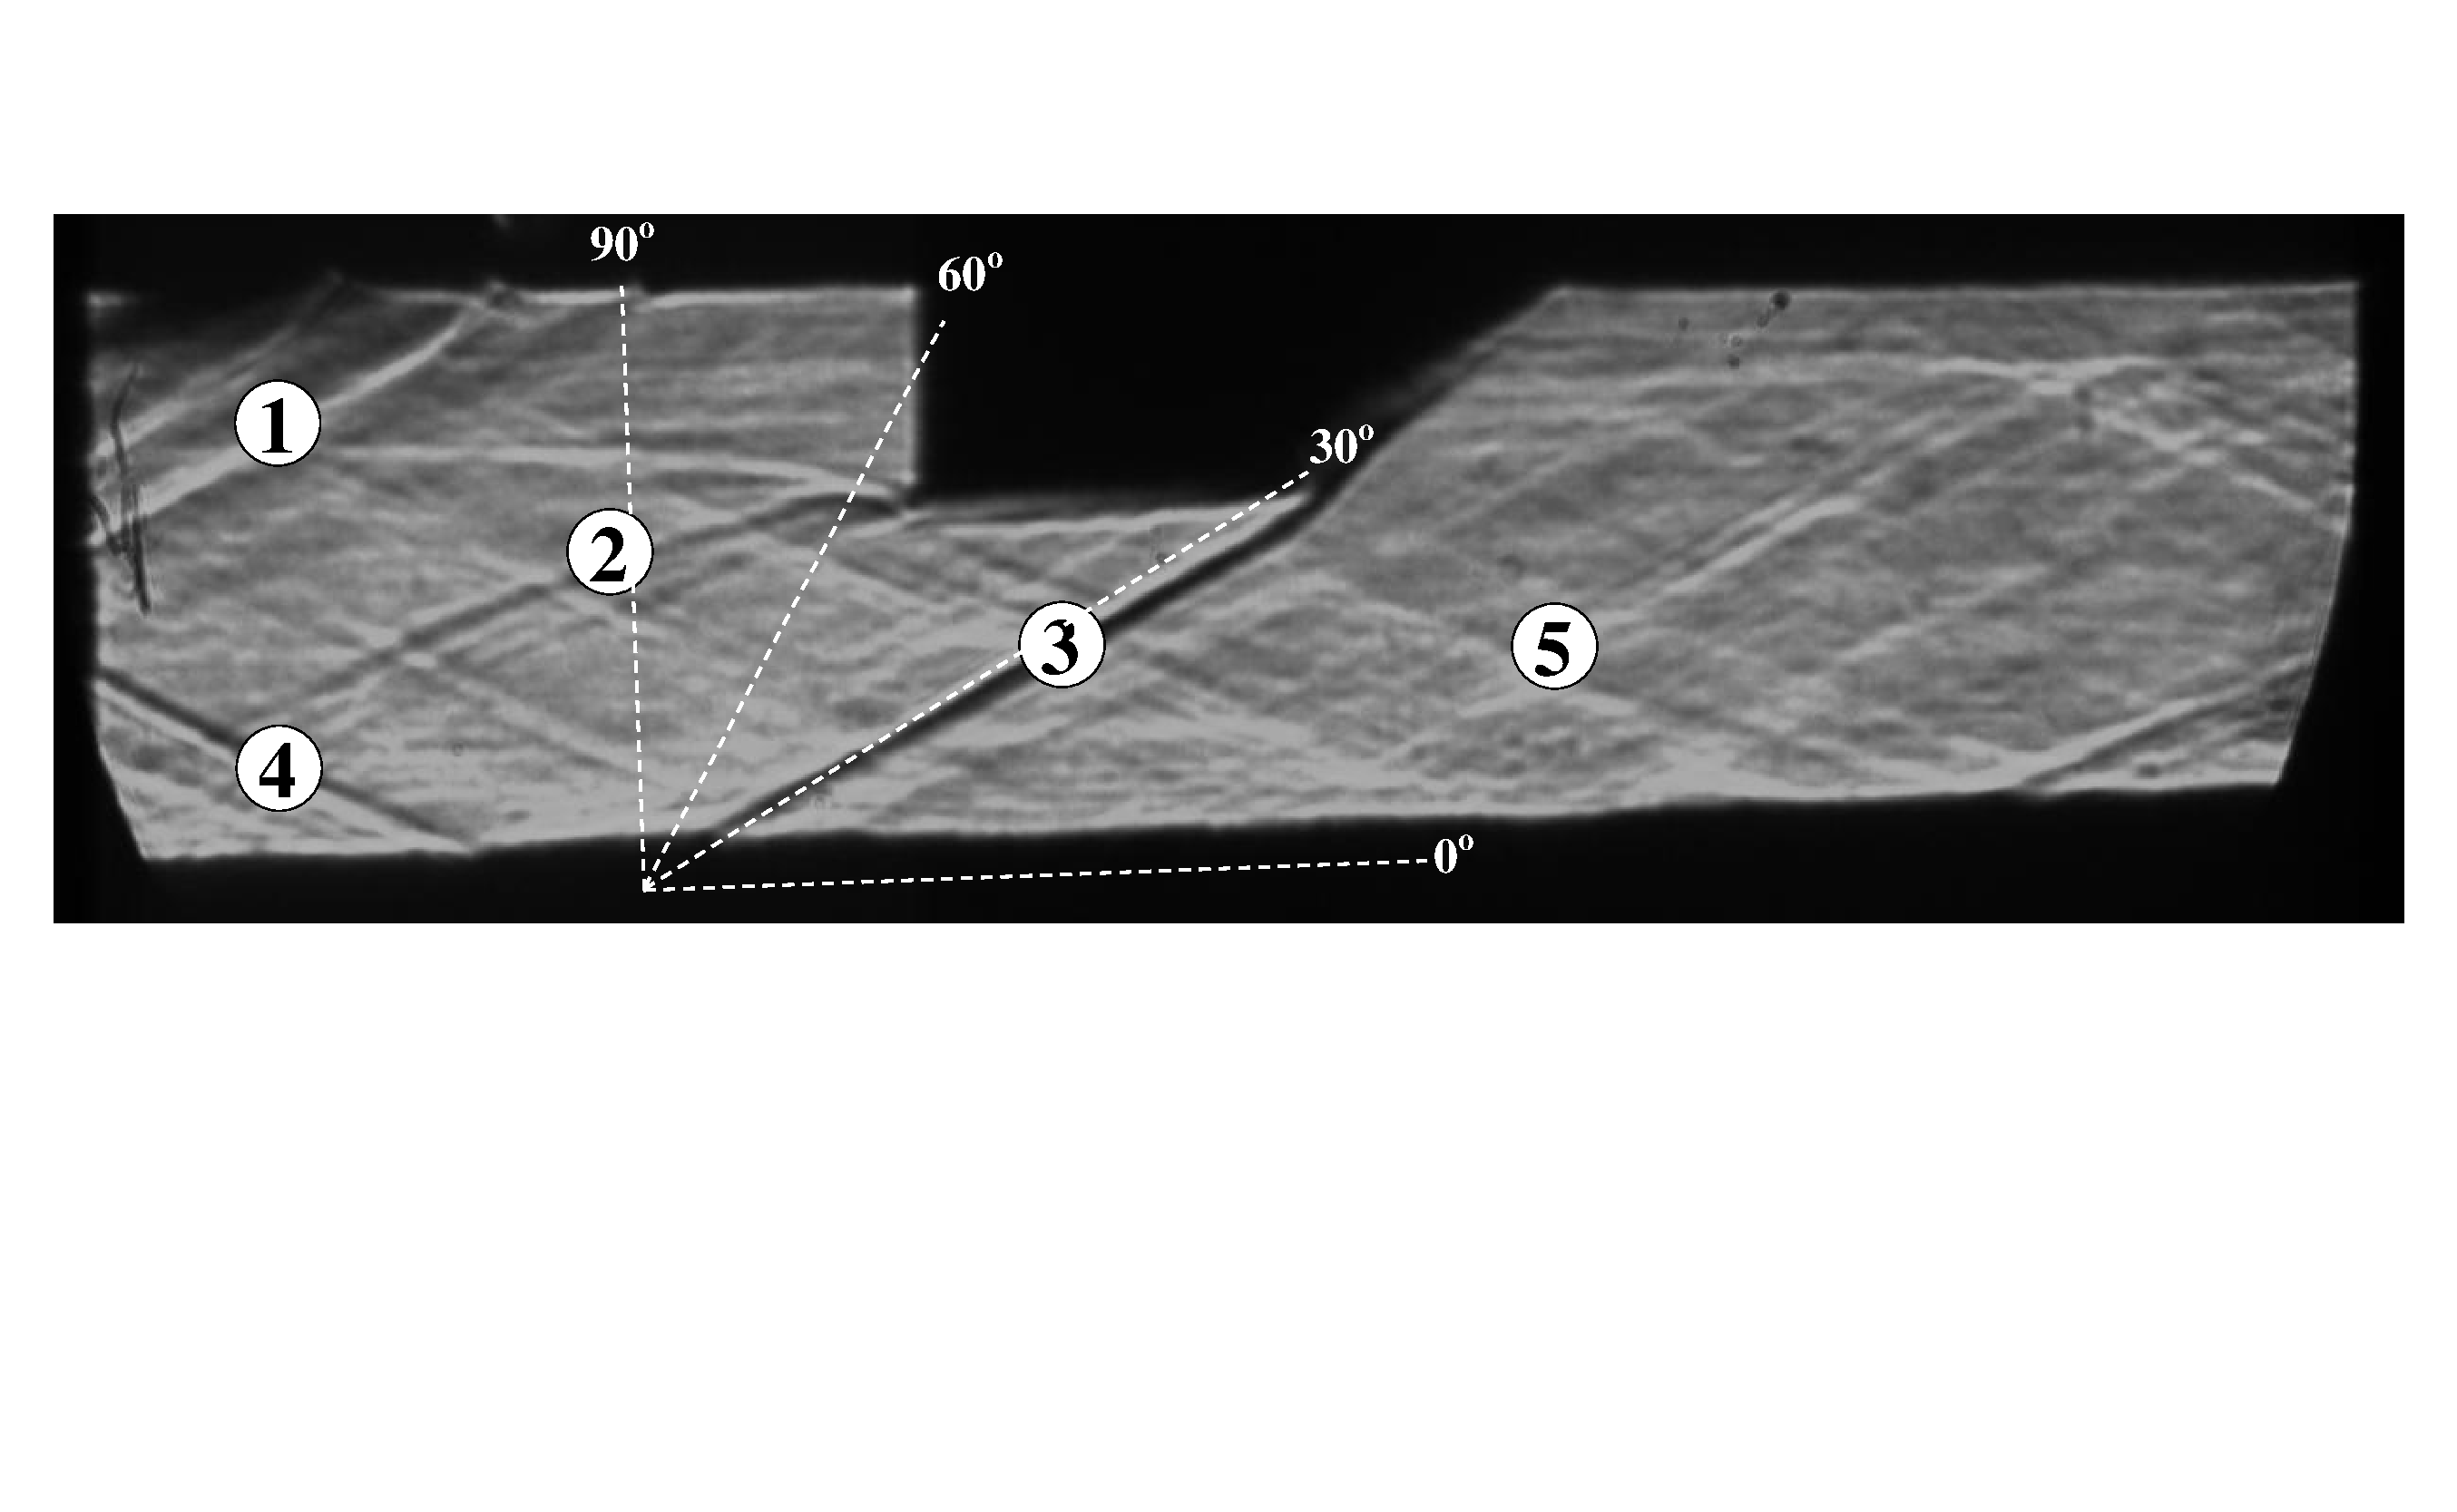
\includegraphics[width=0.95\textwidth]{WaveShadowMarker.pdf}}
\end{center}

\begin{enumerate}
\item 由于燃烧室内流道内壁有突起造成干扰波.
\item 是膨胀波系.
\item 是一个激波.
\item 是3处的激波在壁面的反射波.
\item 前部的壁面扰动与其在风动内部反射的结果.
\end{enumerate}
}


\frame{\frametitle{马赫数分析}
\begin{center}
\fbox{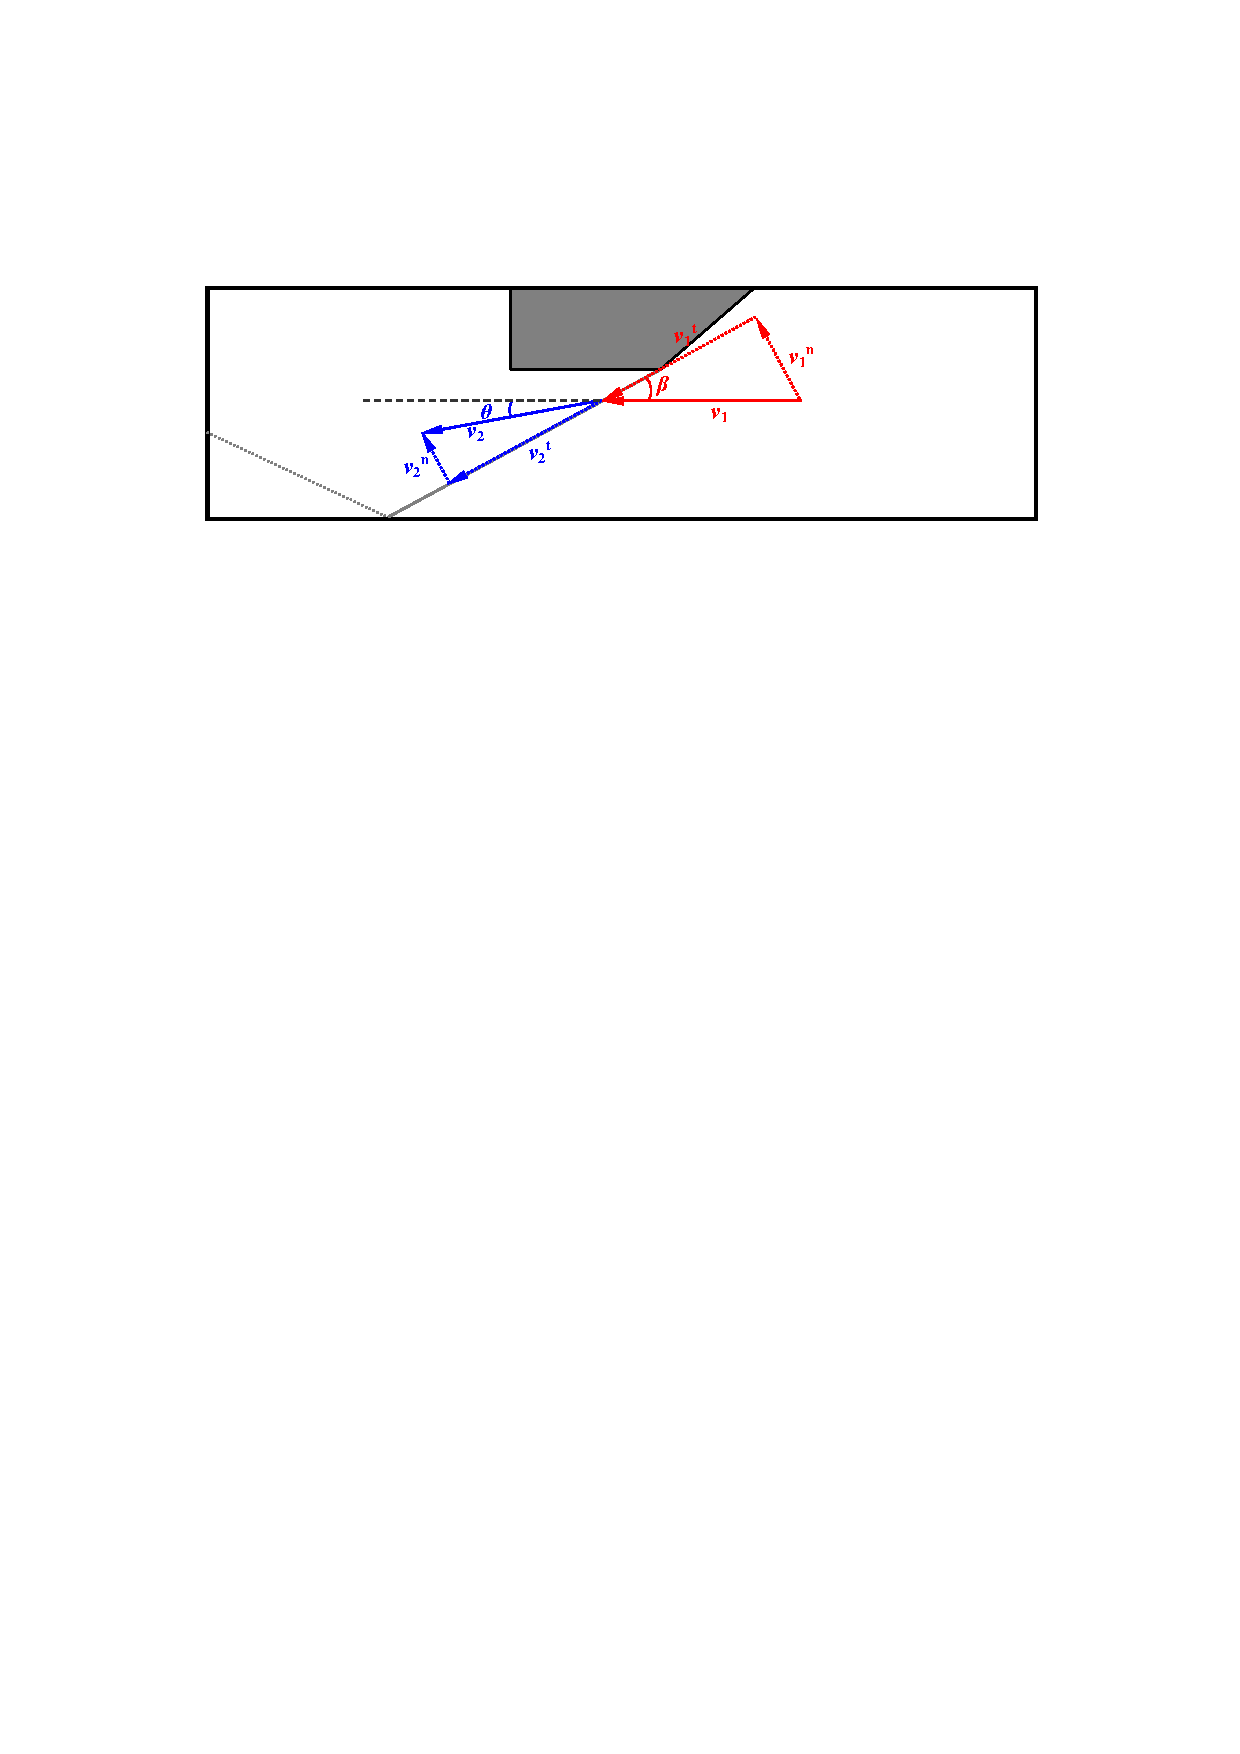
\includegraphics[width=0.95\textwidth]{analysis.pdf}}
\end{center}

{\footnotesize
\[
\tan\beta = v_1^n/v_1^t, \,\,\,\,\,\, \tan(\beta-\theta)=v_2^n/v_1^t, \,\,\,\,\,\, v_1^t = v_2^t
\]
\[
\frac{\tan(\beta-\theta)}{\tan\beta} = \frac{v_2^n}{v_1^n} = \frac{\rho_1}{\rho_2} = \frac{2+(\gamma-1)M_1\sin^2\beta}{(\gamma+1)M_1\sin^2\beta}
\Rightarrow
\tan\theta = \frac{M_1^2\sin^2\beta-1}{M_1^2(\gamma+\cos 2\beta)+2}
\]}
波前波后的速度都应平行壁面, 即$\theta = 0$. 因此$\beta=\pi/2$或$\sin\beta=\frac{1}{M_1}$, 此处应为$\sin\beta=\frac{1}{M_1}$. 可知$\beta\approx\pi/6$, 因此波前马赫数$M_1\approx2$.
}
